\documentclass[a4j]{jarticle}
\usepackage[dvipdfmx]{graphicx}
\usepackage{amssymb}
\usepackage{subfigure}
\usepackage{longtable}

\begin{document}
\begin{table}[t]
\begin{center}
{\large 産業用モニタリングシステムにおける障害検知手法の提案}\\
令和 2 年 8 月 4 日\\
山本 航平
\end{center}
\end{table}

進捗報告
\begin{itemize}
\item FTP を用いない一日を通じた 15 秒間隔での計測実験を終えました.
\item FTP を用いた計測実験の準備を進めています.
\item 一日を通じた計測実験で見られる,低遅延帯が時間経過に伴い増加傾向を示す区間の時間的長さを調べました.
\item 大きな応答遅延の発生要因箇所の切り分けを行いました.
\end{itemize}
\section{FTP を用いない計測データ}
6 月 23 日(火)から 7 月 22 日(水)までの約一か月間,一日を通じ 15 秒間隔で ping による応答遅延を計測した.
この計測により得られた各計測時刻における ping 応答遅延の値を一日ごとにわけて図 \ref{all1} と図 \ref{all2} に示す.
また,赤色点線はその時刻に Raspberry Pi の LTE 接続が切れたことを表す.
また,7 月 7 日 と 7 月 15 日から 7 月 16 日にかけての一部区間の計測データが損なわれているが,これは私の行った作業によるものであり通信障害によるものではない.
図 \ref{all1} と図 \ref{all2} より,応答遅延はほとんどが 60 ミリ秒から 90 ミリ秒までの値をとるようだが,時折より大きな値を取るようだ.この大きな応答遅延の発生頻度は 6 月 25 日や 7 月 10 日のように高い区間もあれば,7 月 1 日のように低い区間もあった.
今後,この発生頻度やその間隔に共通性や差異が見られないか分析を行う予定である.
\begin{figure}[tb]
\begin{center}
\subfigure[6 月 23 日(火)]{
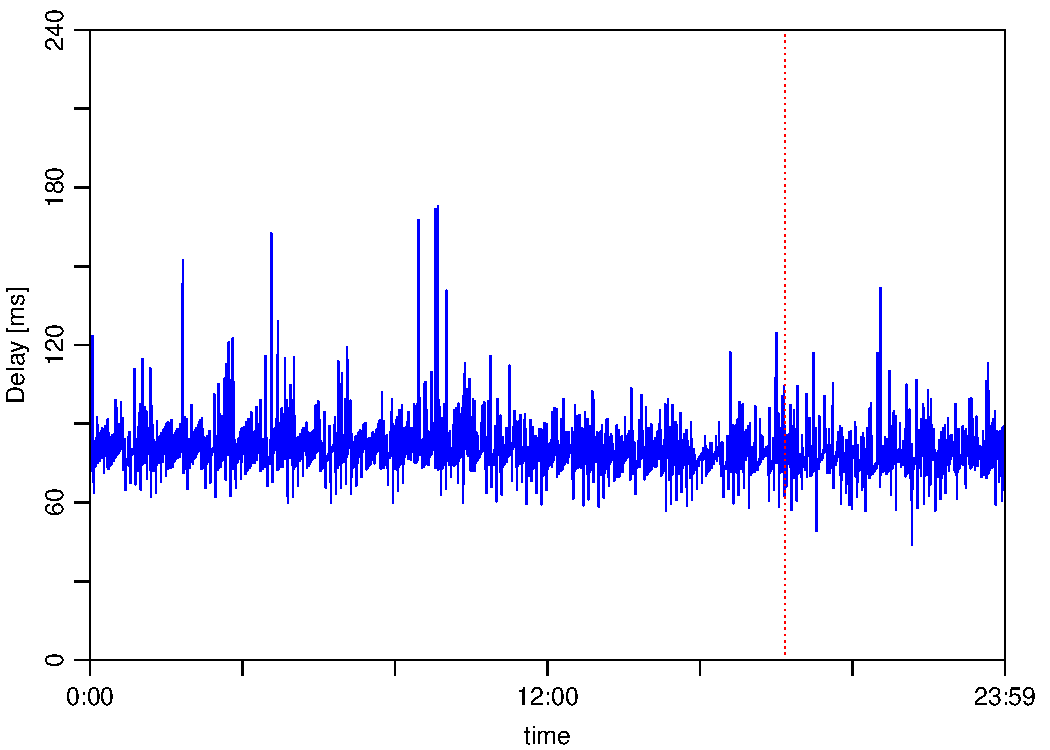
\includegraphics[width=0.33\hsize]{C:/master/mstudy/analysis/long/plot-6-23.pdf}
}~
\subfigure[6 月 24 日(水)]{
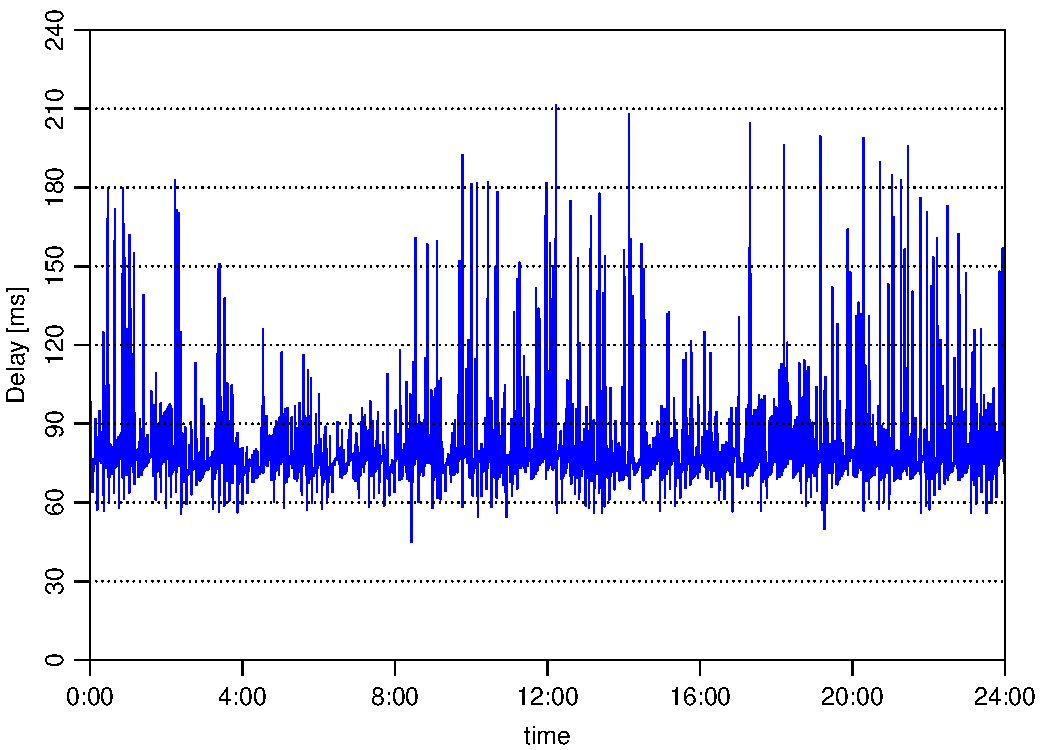
\includegraphics[width=0.33\hsize]{C:/master/mstudy/analysis/long/plot-6-24.pdf}
}~
\subfigure[6 月 25 日(木)]{
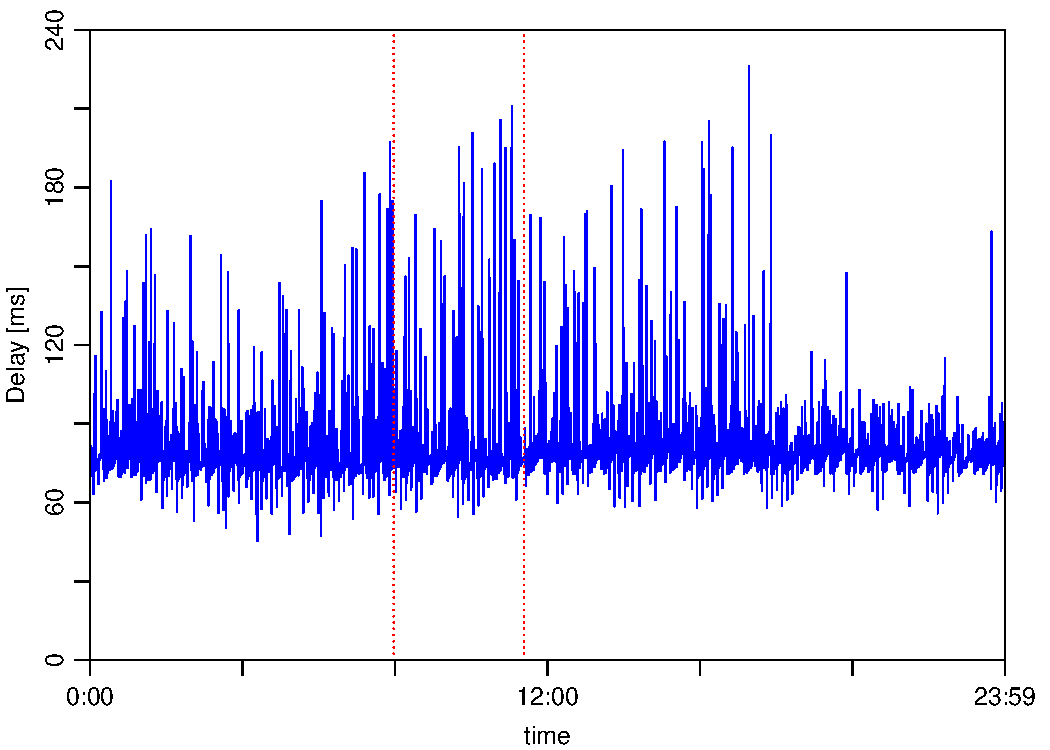
\includegraphics[width=0.33\hsize]{C:/master/mstudy/analysis/long/plot-6-25.pdf}
}\\
\subfigure[6 月 26 日(金)]{
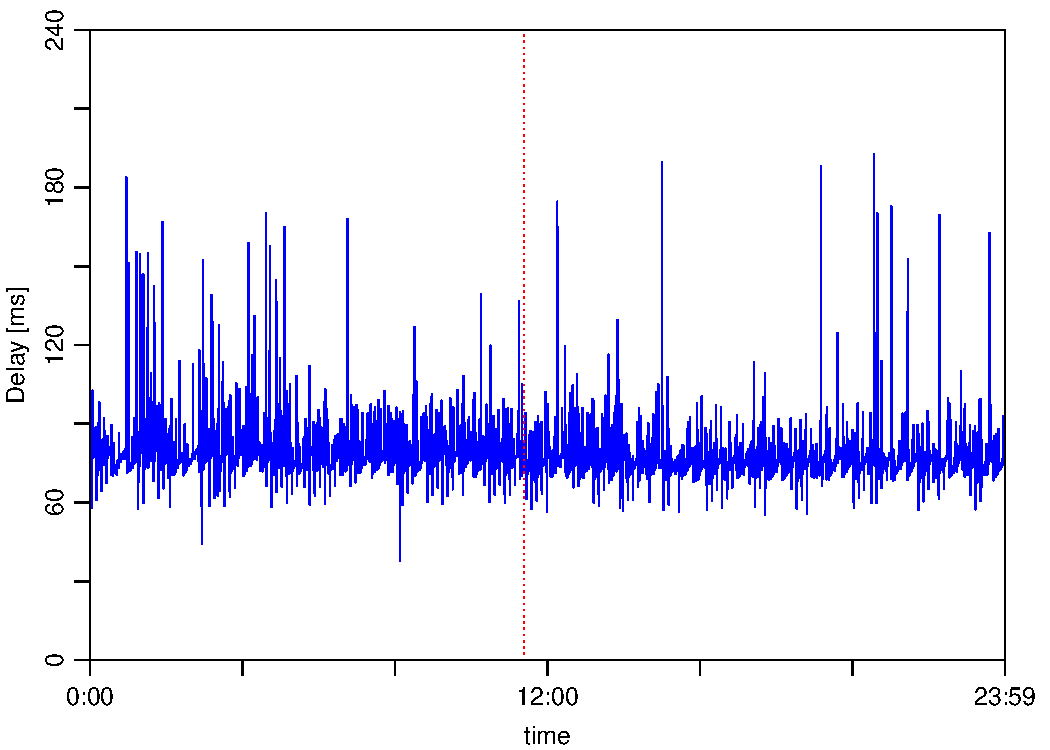
\includegraphics[width=0.33\hsize]{C:/master/mstudy/analysis/long/plot-6-26.pdf}
}~
\subfigure[6 月 27 日(土)]{
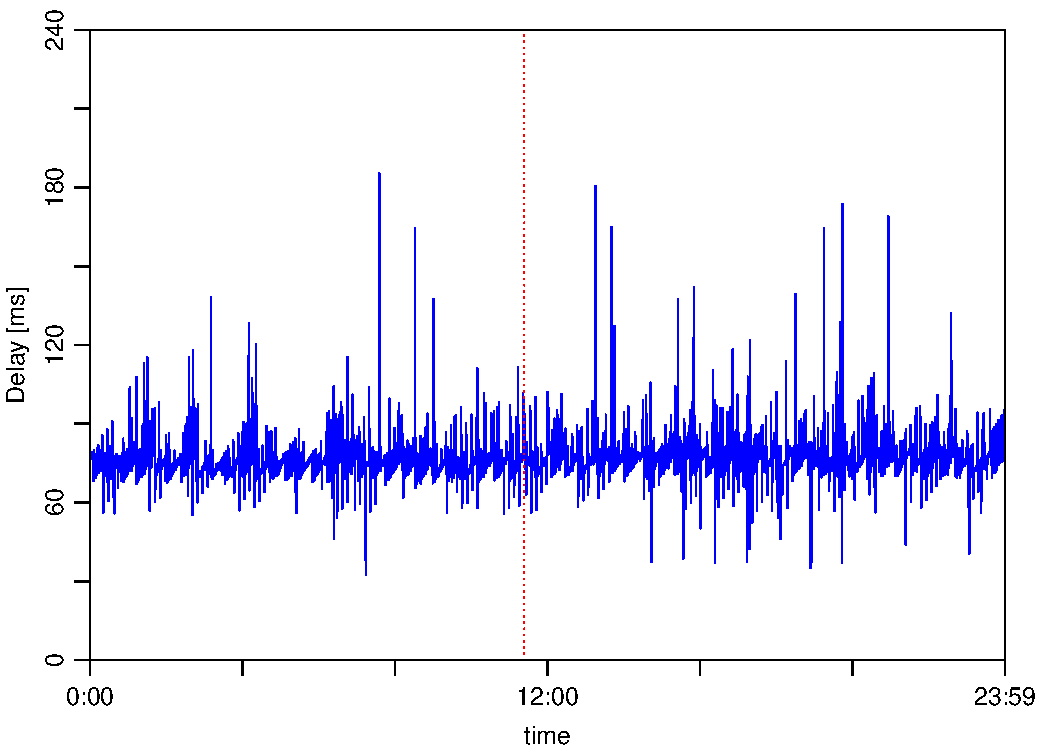
\includegraphics[width=0.33\hsize]{C:/master/mstudy/analysis/long/plot-6-27.pdf}
}~
\subfigure[6 月 28 日(日)]{
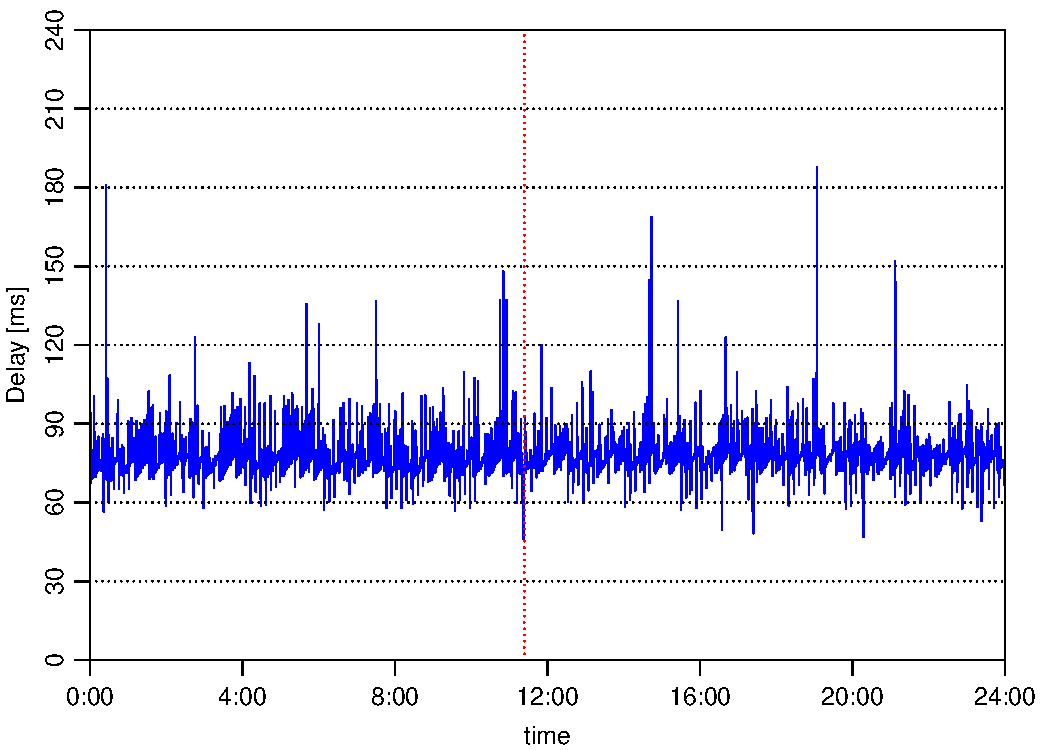
\includegraphics[width=0.33\hsize]{C:/master/mstudy/analysis/long/plot-6-28.pdf}
}\\
\subfigure[6 月 29 日(月)]{
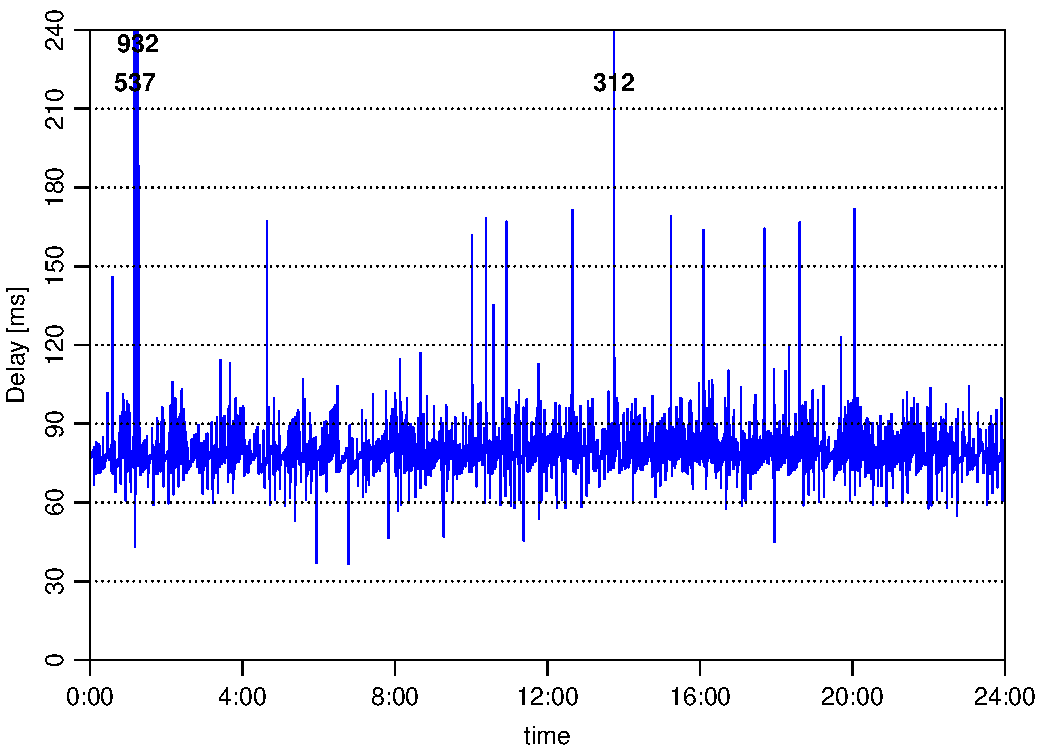
\includegraphics[width=0.33\hsize]{C:/master/mstudy/analysis/long/plot-6-29.pdf}
}~
\subfigure[6 月 30 日(火)]{
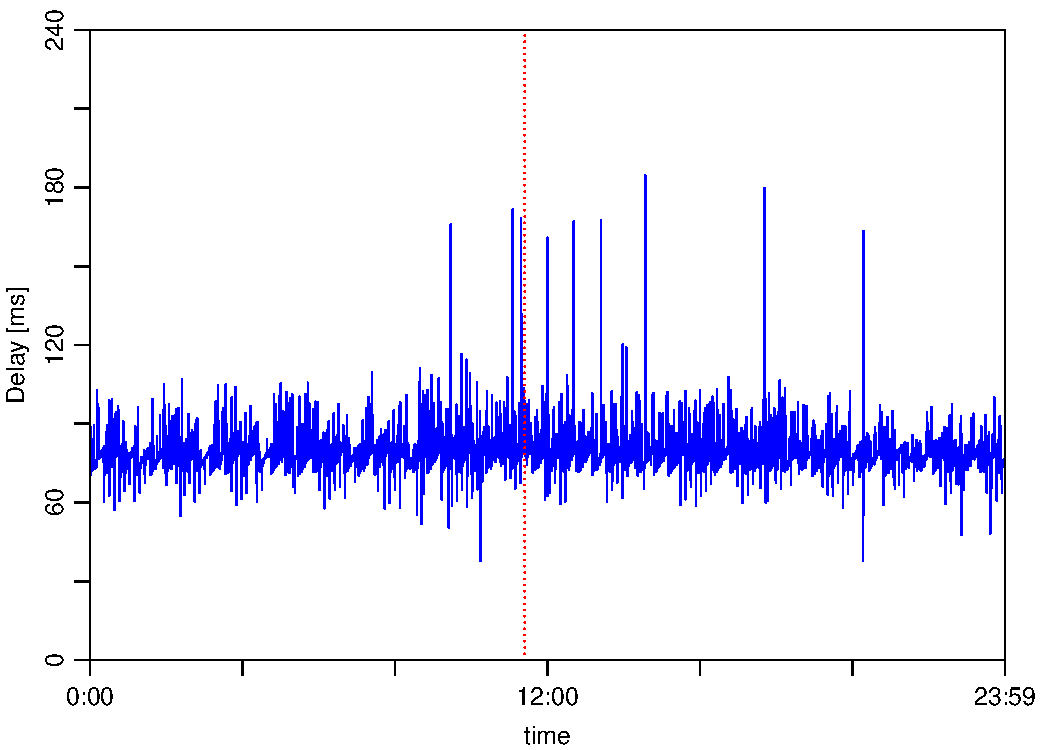
\includegraphics[width=0.33\hsize]{C:/master/mstudy/analysis/long/plot-6-30.pdf}
}~
\subfigure[7 月 1 日(水)]{
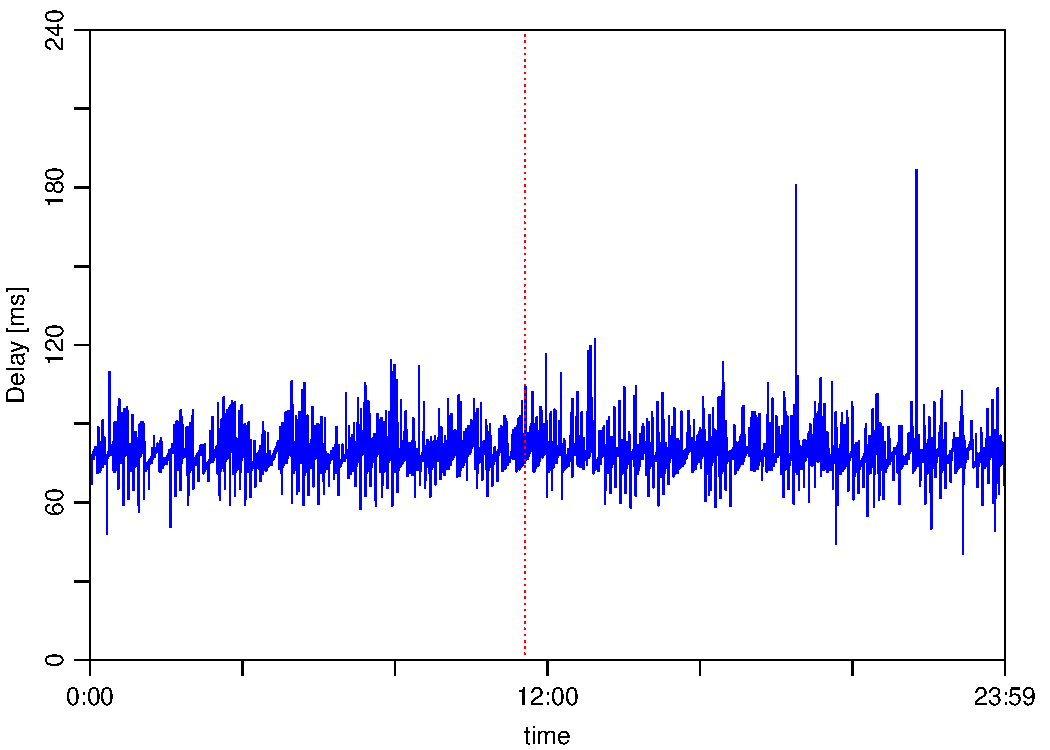
\includegraphics[width=0.33\hsize]{C:/master/mstudy/analysis/long/plot-7-1.pdf}
}\\
\subfigure[7 月 2 日(木)]{
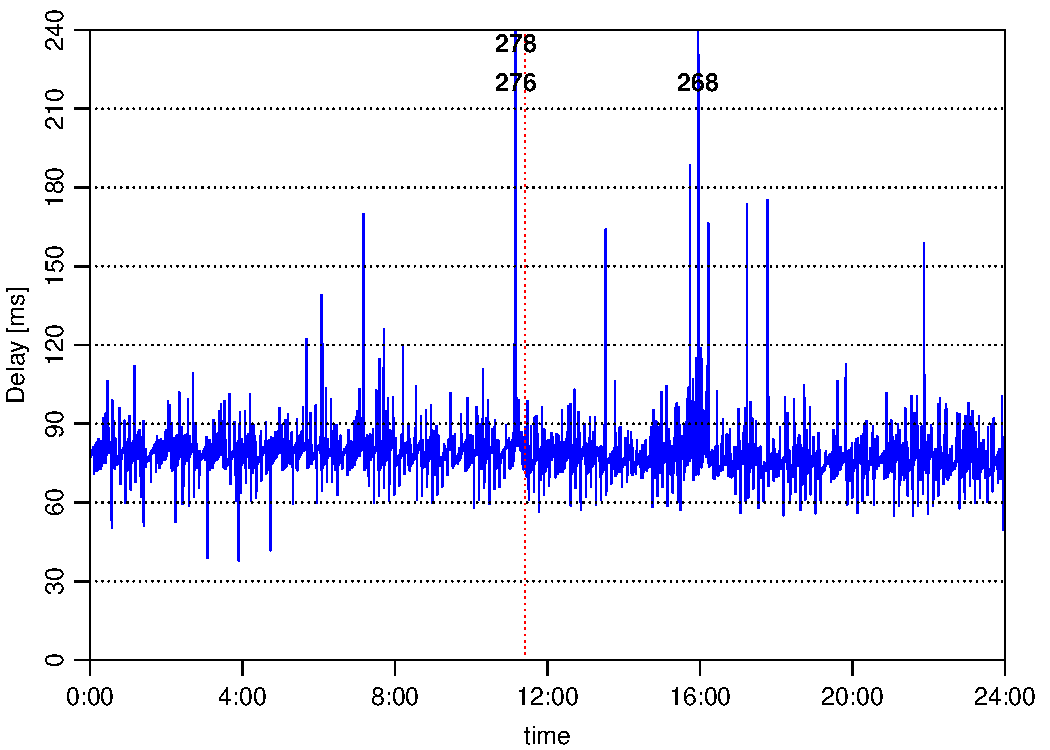
\includegraphics[width=0.33\hsize]{C:/master/mstudy/analysis/long/plot-7-2.pdf}
}~
\subfigure[7 月 3 日(金)]{
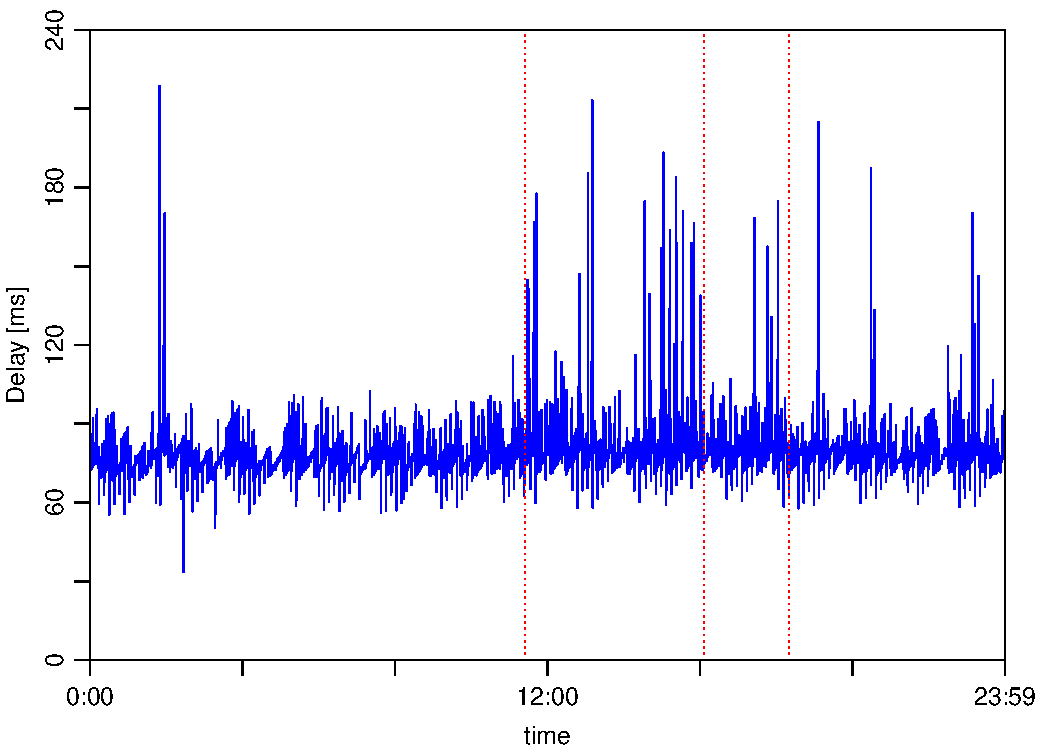
\includegraphics[width=0.33\hsize]{C:/master/mstudy/analysis/long/plot-7-3.pdf}
}~
\subfigure[7 月 4 日(土)]{
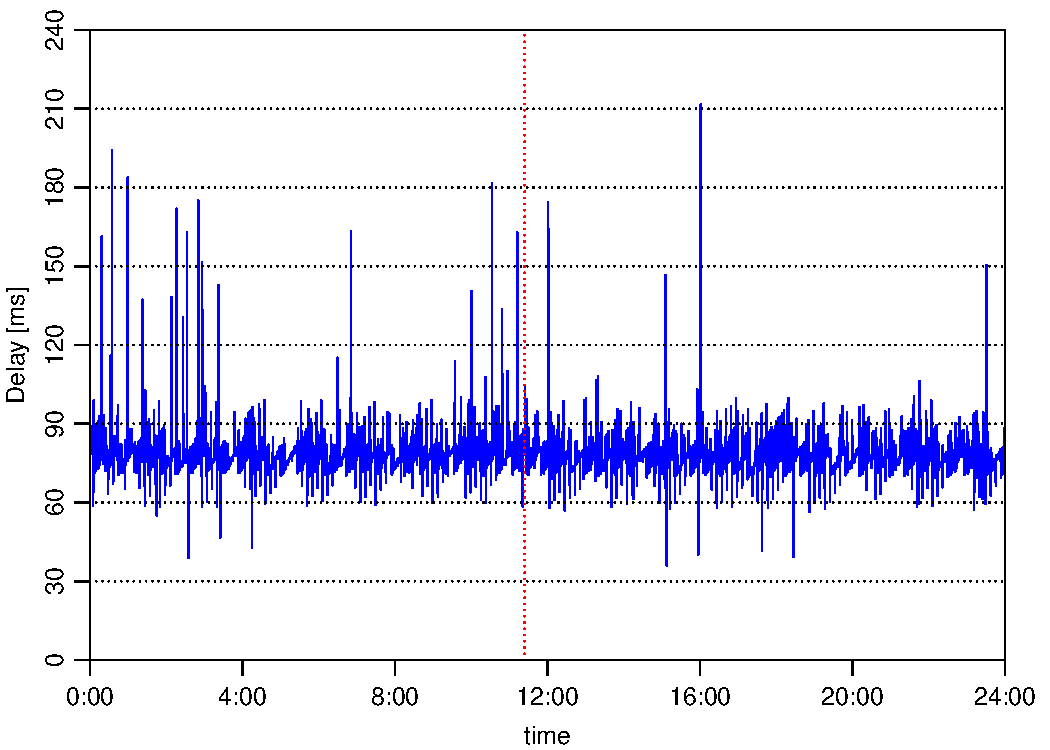
\includegraphics[width=0.33\hsize]{C:/master/mstudy/analysis/long/plot-7-4.pdf}
}\\
\subfigure[7 月 5 日(日)]{
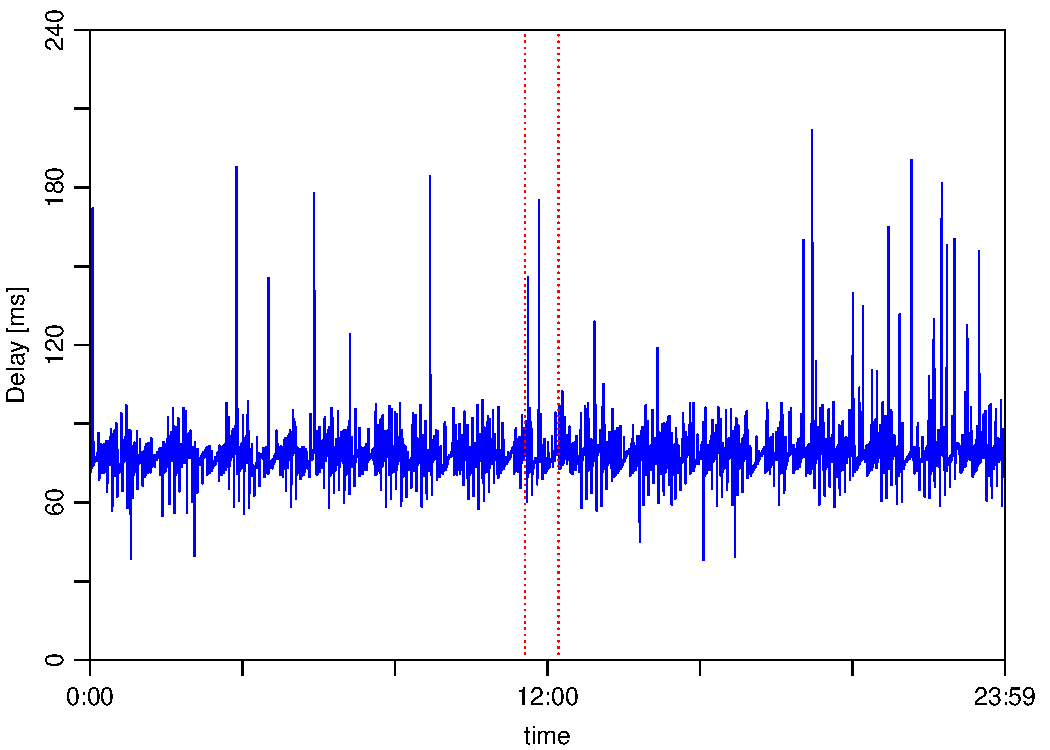
\includegraphics[width=0.33\hsize]{C:/master/mstudy/analysis/long/plot-7-5.pdf}
}~
\subfigure[7 月 6 日(月)]{
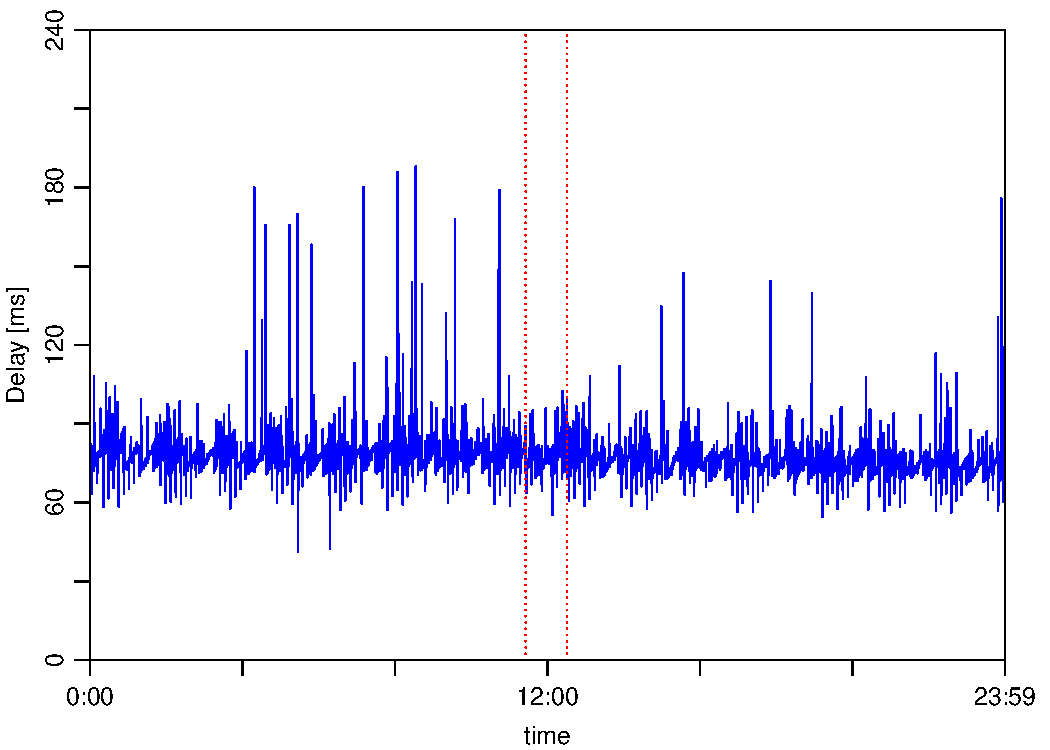
\includegraphics[width=0.33\hsize]{C:/master/mstudy/analysis/long/plot-7-6.pdf}
}~
\subfigure[7 月 7 日(火)]{
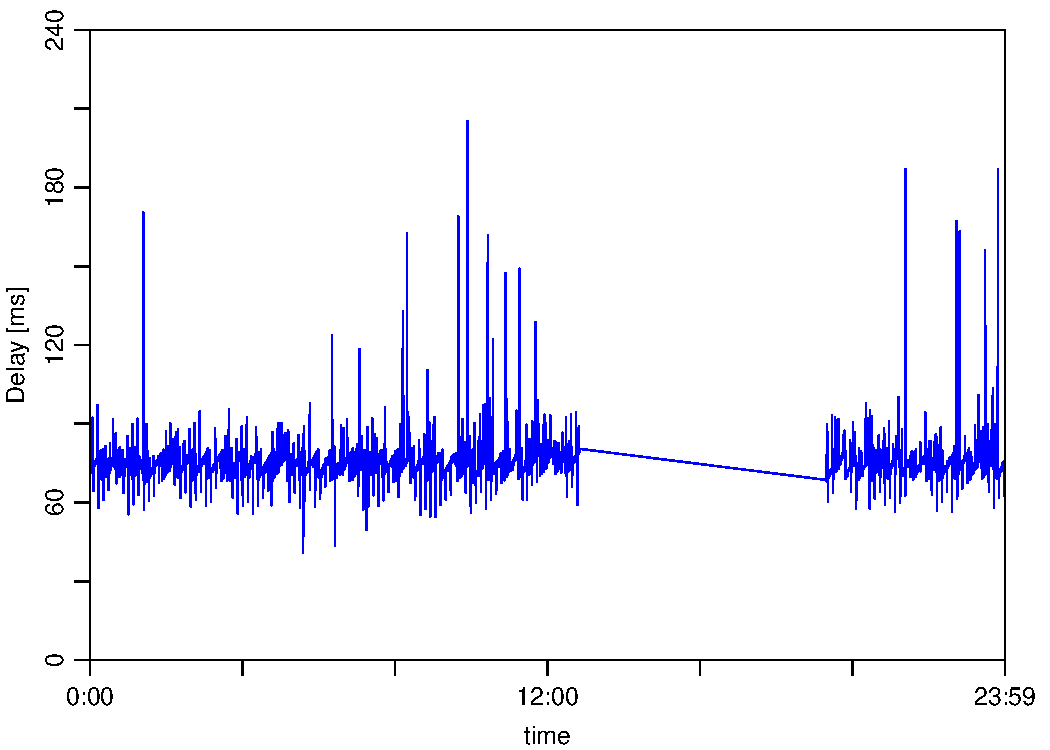
\includegraphics[width=0.33\hsize]{C:/master/mstudy/analysis/long/plot-7-7.pdf}
}
\caption{計測結果(6 月 23 日から 7 月 7 日まで)}
\label{all1}
\end{center}
\end{figure}
\begin{figure}[tb]
\begin{center}
\subfigure[7 月 8 日(水)]{
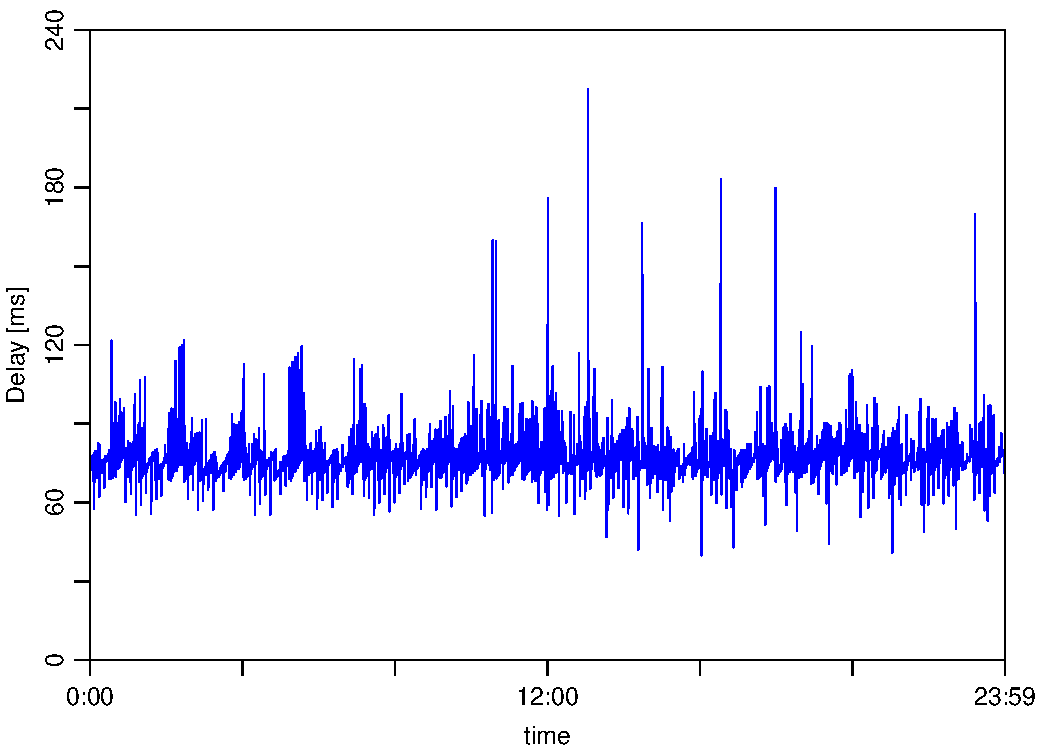
\includegraphics[width=0.33\hsize]{C:/master/mstudy/analysis/long/plot-7-8.pdf}
}~
\subfigure[7 月 9 日(木)]{
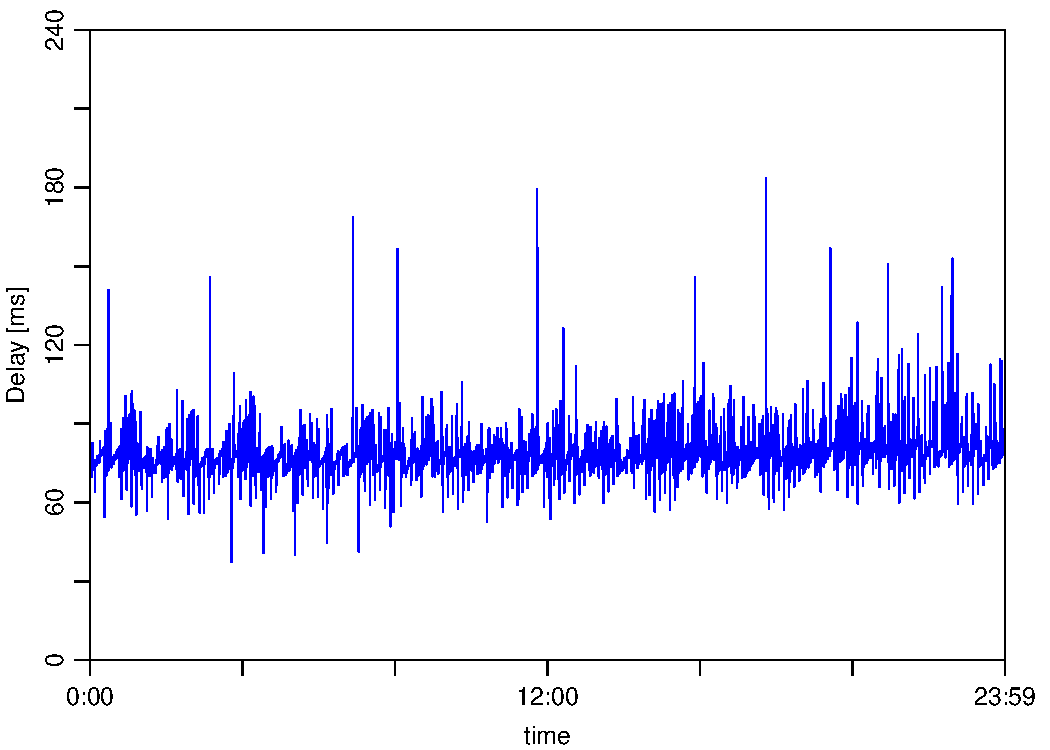
\includegraphics[width=0.33\hsize]{C:/master/mstudy/analysis/long/plot-7-9.pdf}
}~
\subfigure[7 月 10 日(金)]{
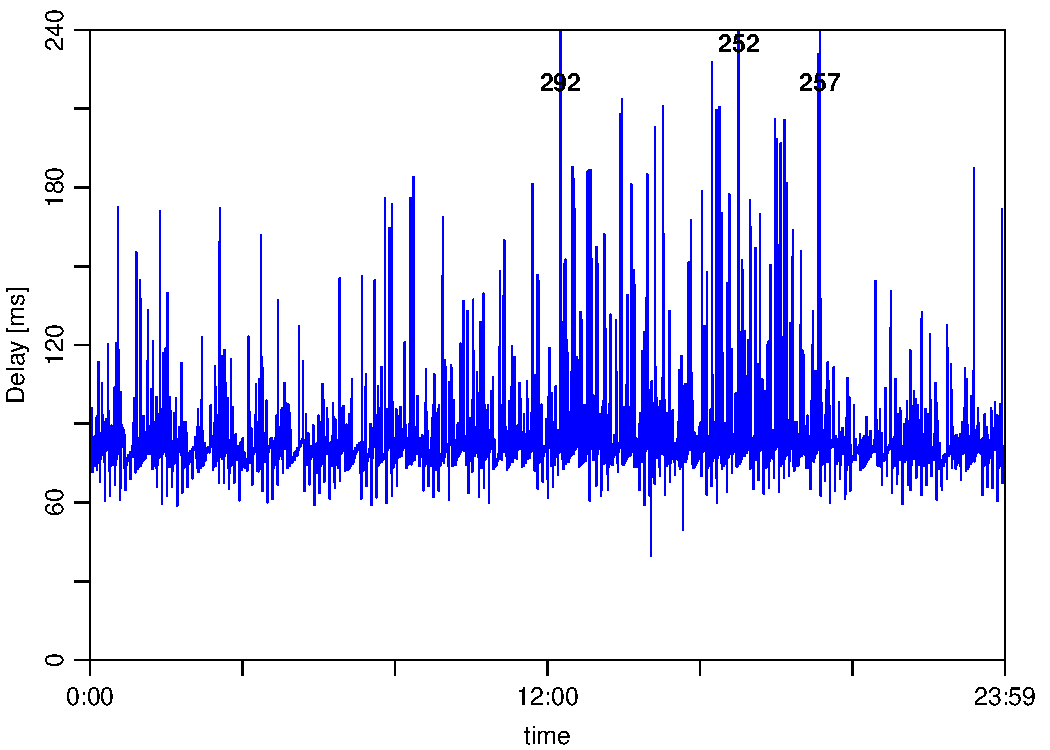
\includegraphics[width=0.33\hsize]{C:/master/mstudy/analysis/long/plot-7-10.pdf}
}\\
\subfigure[7 月 11 日(土)]{
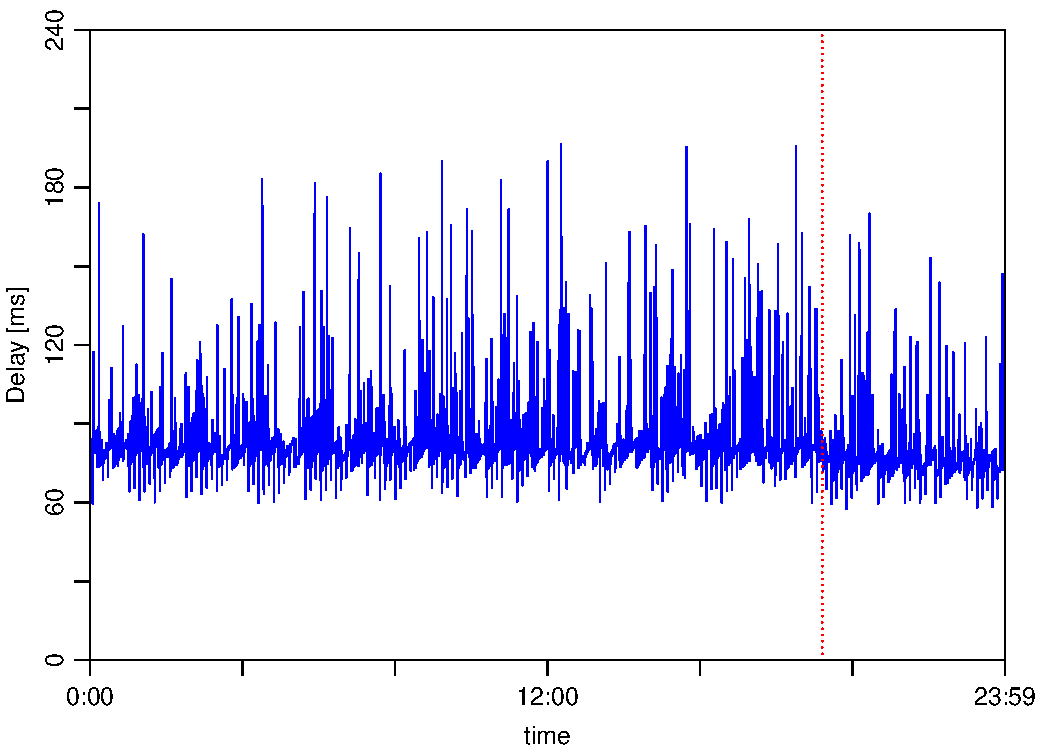
\includegraphics[width=0.33\hsize]{C:/master/mstudy/analysis/long/plot-7-11.pdf}
}~
\subfigure[7 月 12 日(日)]{
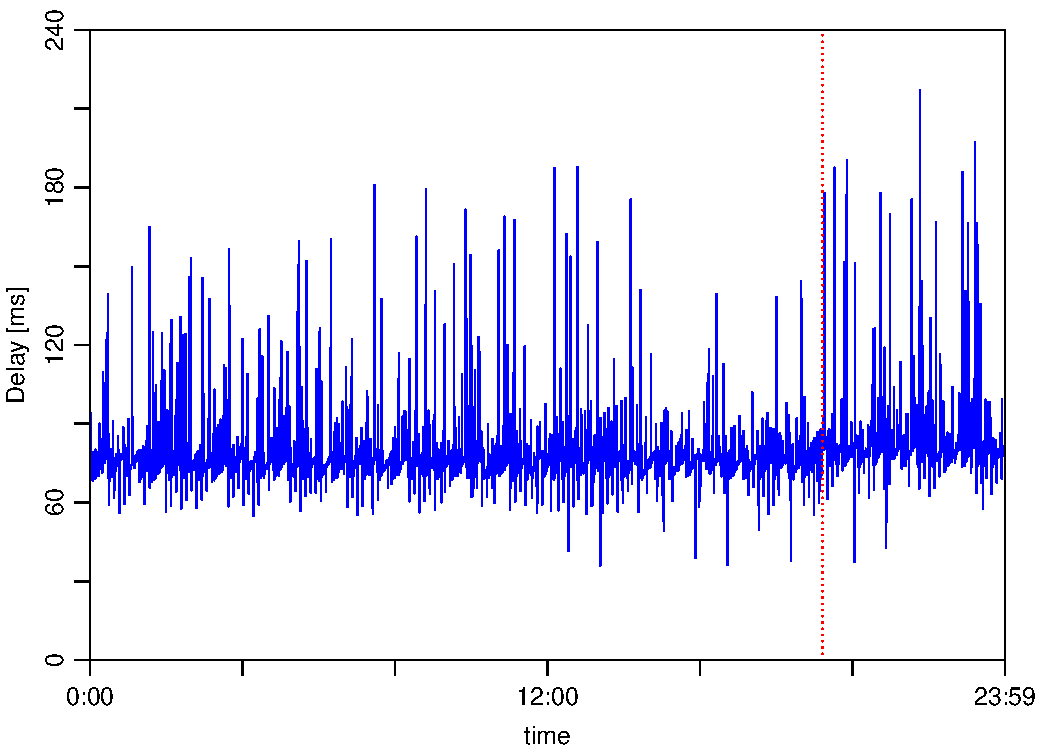
\includegraphics[width=0.33\hsize]{C:/master/mstudy/analysis/long/plot-7-12.pdf}
}~
\subfigure[7 月 13 日(月)]{
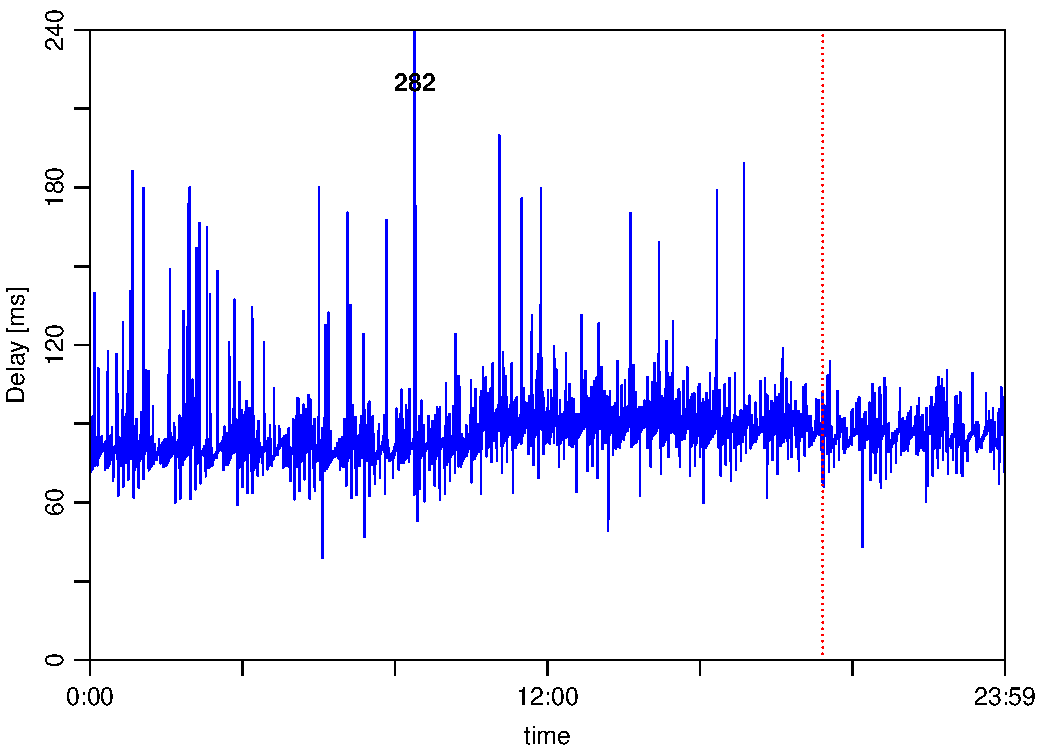
\includegraphics[width=0.33\hsize]{C:/master/mstudy/analysis/long/plot-7-13.pdf}
}\\
\subfigure[7 月 14 日(火)]{
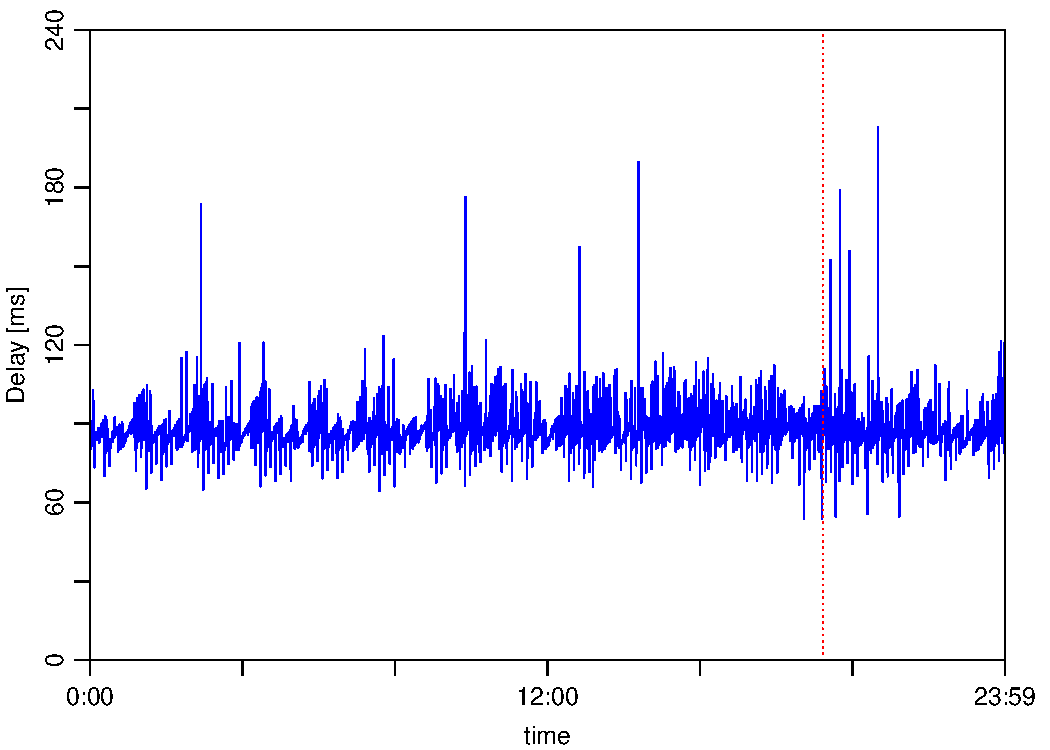
\includegraphics[width=0.33\hsize]{C:/master/mstudy/analysis/long/plot-7-14.pdf}
}~
\subfigure[7 月 15 日(水)]{
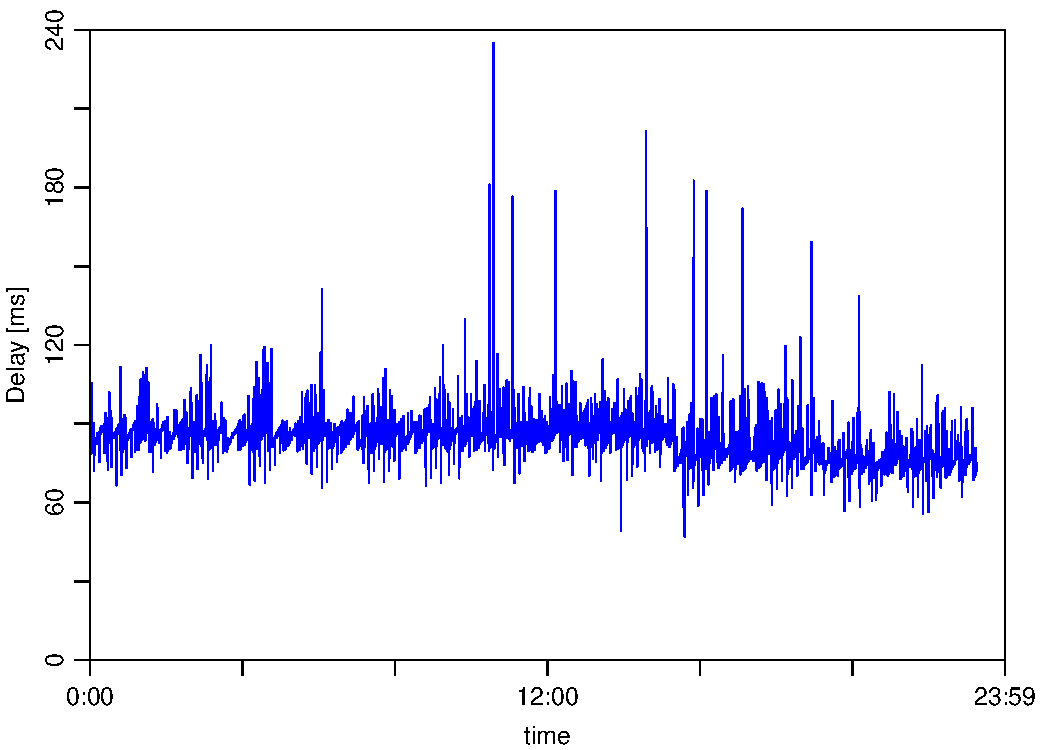
\includegraphics[width=0.33\hsize]{C:/master/mstudy/analysis/long/plot-7-15.pdf}
}~
\subfigure[7 月 16 日(木)]{
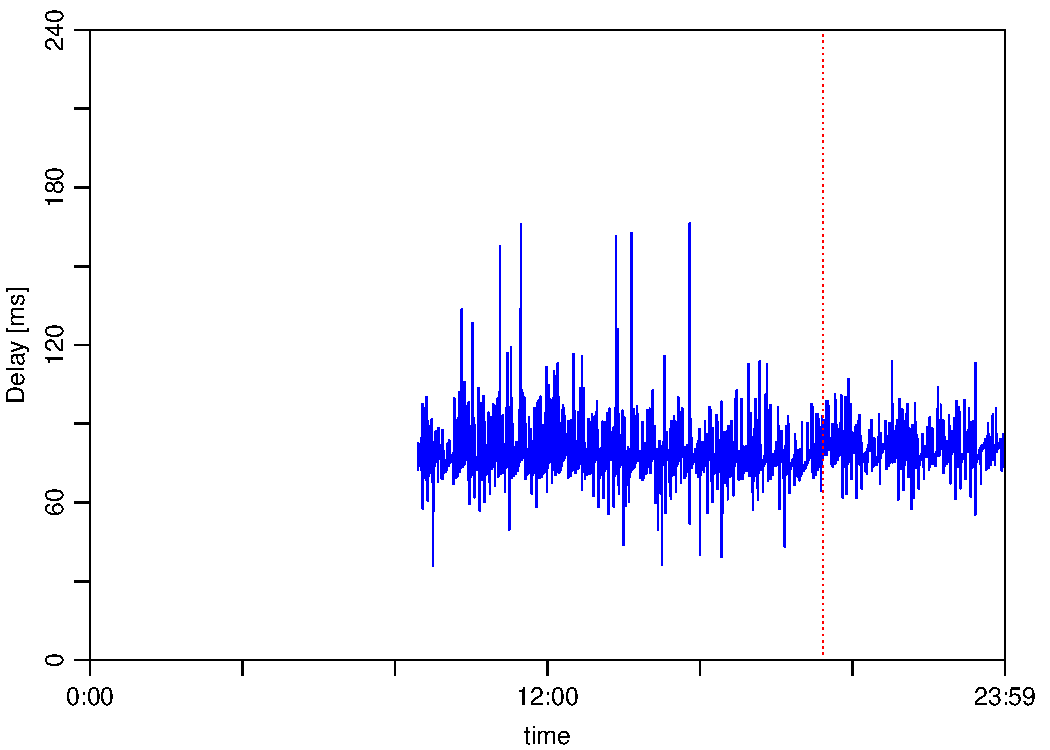
\includegraphics[width=0.33\hsize]{C:/master/mstudy/analysis/long/plot-7-16.pdf}
}\\
\subfigure[7 月 17 日(金)]{
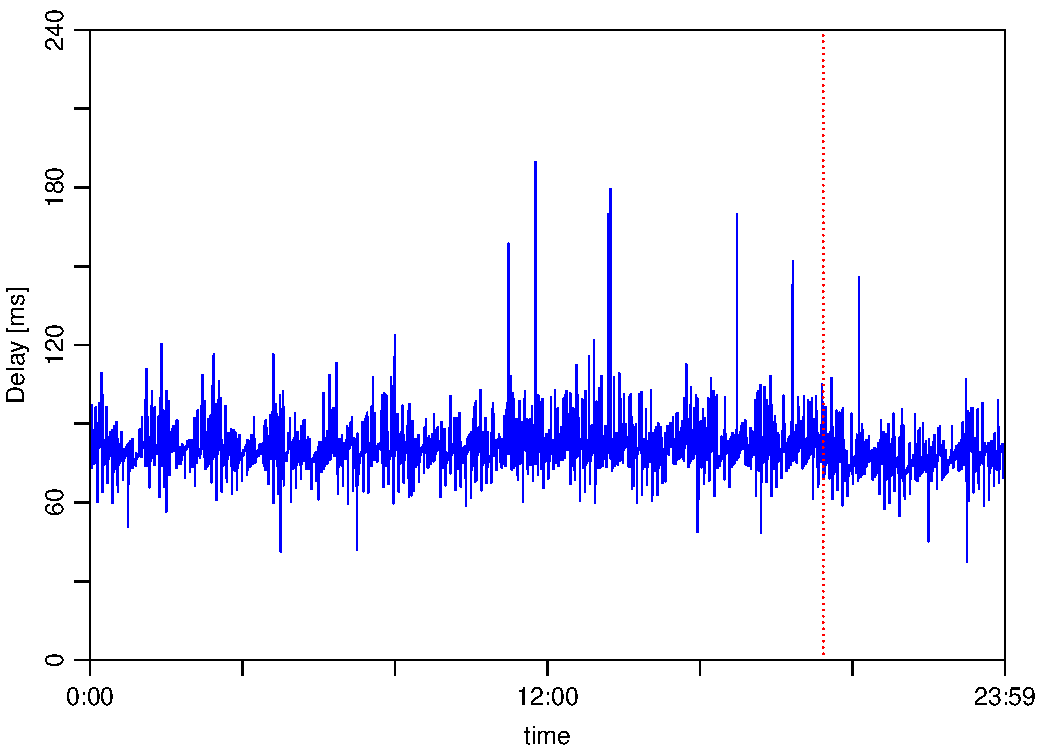
\includegraphics[width=0.33\hsize]{C:/master/mstudy/analysis/long/plot-7-17.pdf}
}~
\subfigure[7 月 18 日(土)]{
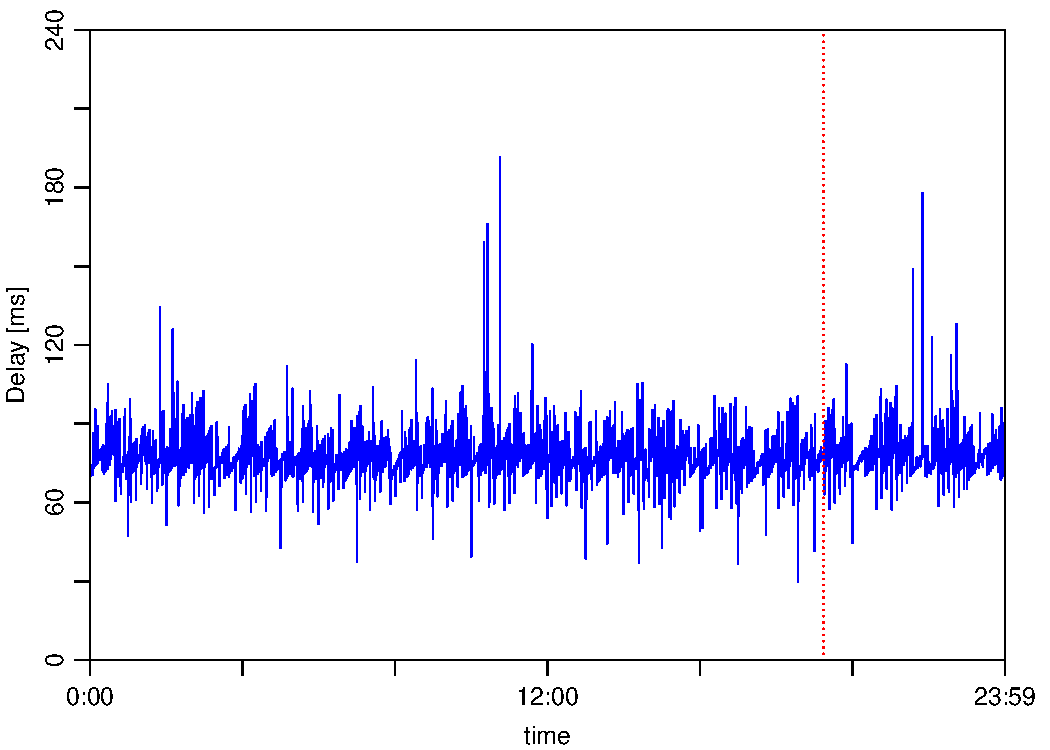
\includegraphics[width=0.33\hsize]{C:/master/mstudy/analysis/long/plot-7-18.pdf}
}~
\subfigure[7 月 19 日(日)]{
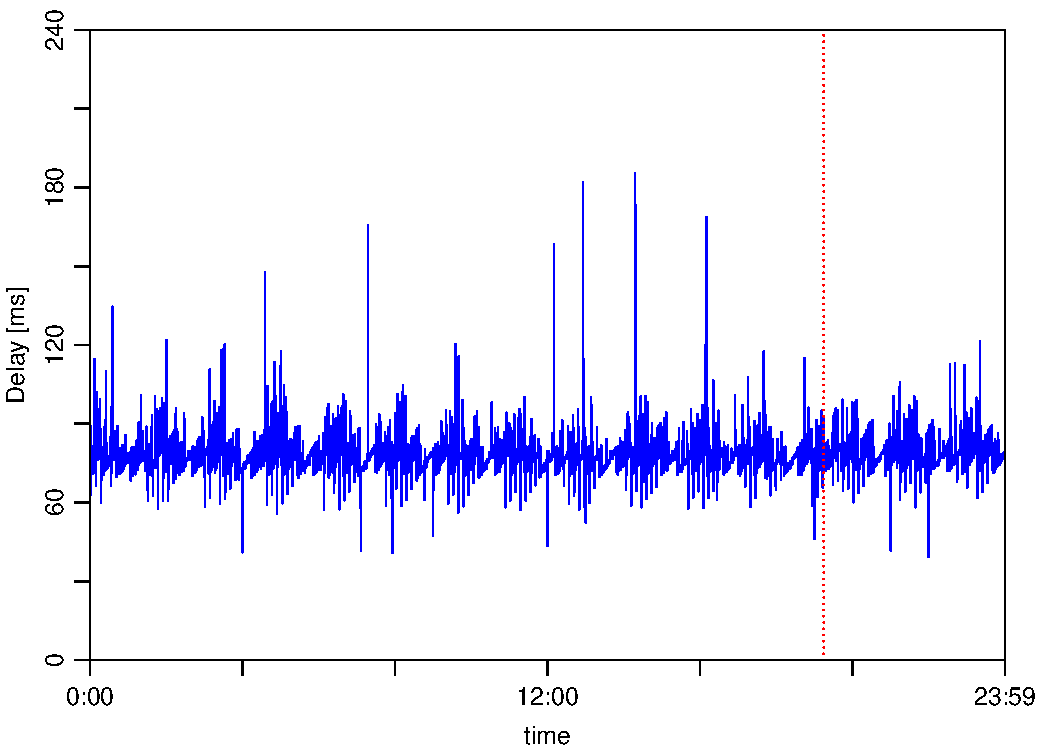
\includegraphics[width=0.33\hsize]{C:/master/mstudy/analysis/long/plot-7-19.pdf}
}\\
\subfigure[7 月 20 日(月)]{
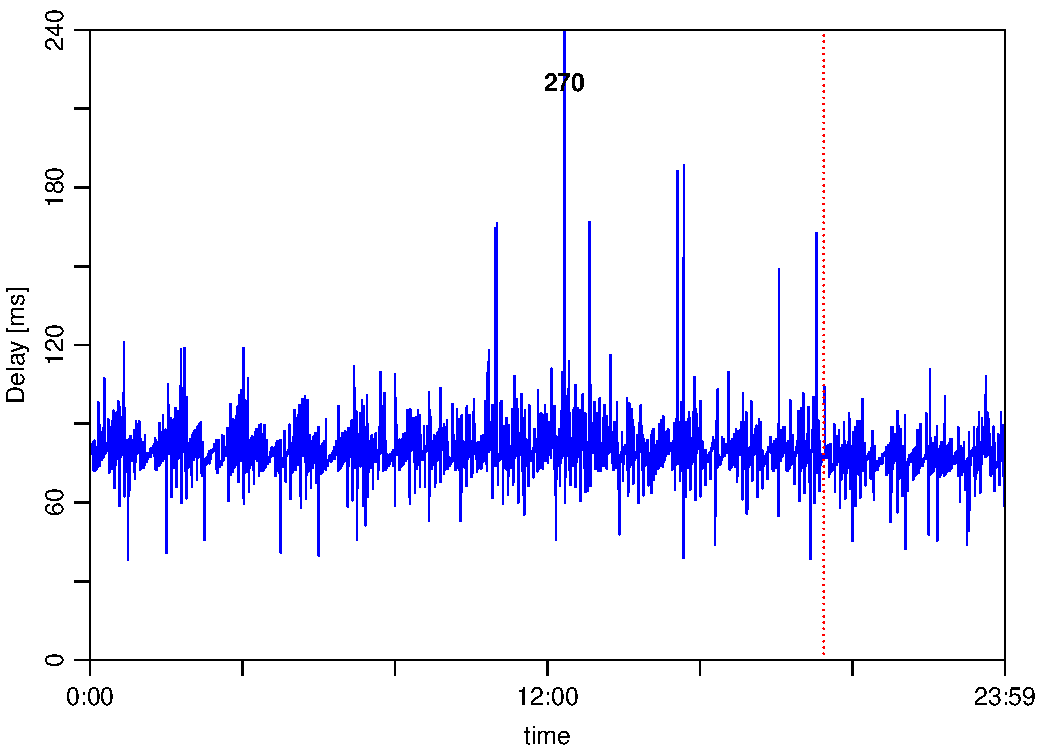
\includegraphics[width=0.33\hsize]{C:/master/mstudy/analysis/long/plot-7-20.pdf}
}~
\subfigure[7 月 21 日(火)]{
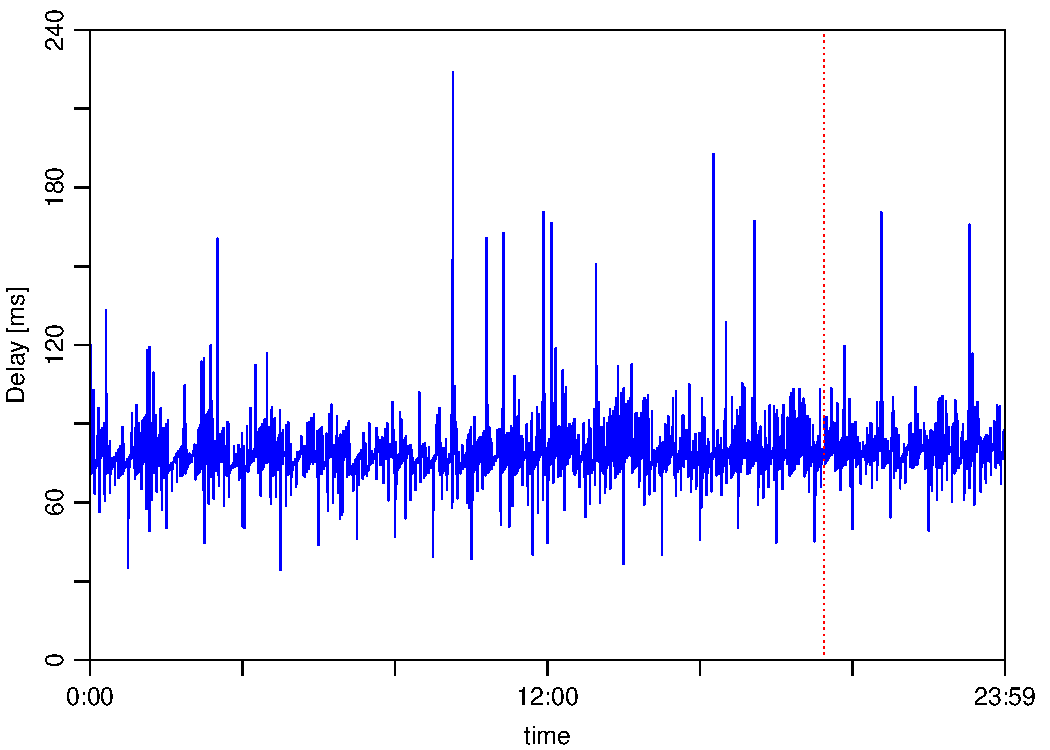
\includegraphics[width=0.33\hsize]{C:/master/mstudy/analysis/long/plot-7-21.pdf}
}~
\subfigure[7 月 22 日(水)]{
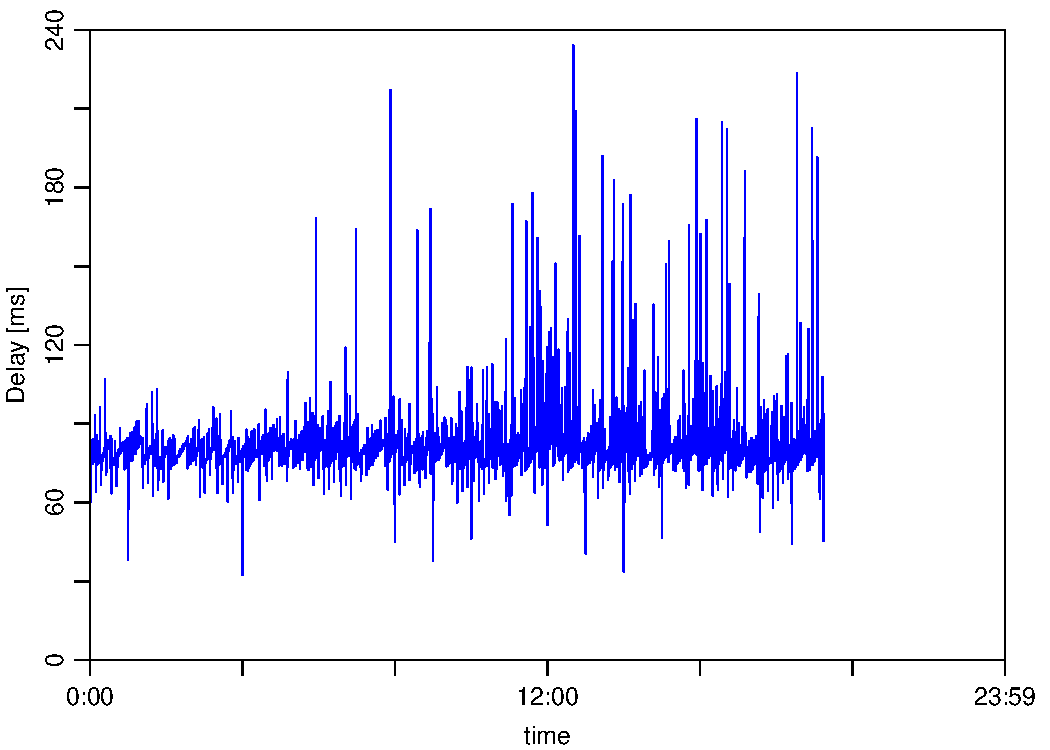
\includegraphics[width=0.33\hsize]{C:/master/mstudy/analysis/long/plot-7-22.pdf}
}
\caption{計測結果(7 月 8 日から 7 月 22 日まで)}
\label{all2}
\end{center}
\end{figure}
\section{FTP を用いた計測実験の進捗}
完了したこと
\begin{itemize}
\item Raspberry Pi のグローバル IP アドレスが AWS サーバとの FTP 通信が可能なアドレス空間に収まるまで再起動によるグローバル IP アドレスの取得を繰り返すこと
\item AWS サーバへのファイル送信(受信)
\item ネットワークが混雑していると考えられる昼間 12 時ごろに 1M バイトのファイルを送信するのにかかった時間は約 4 秒でした.裏で FTP によるファイル送信を実行した状況で 1 時間計測を行うとすると,単純計算で送信ファイルサイズは約 900 MB必要になる.契約中の SIM カードの通信速度制限が 3GB なので,FTP を用いた実験は計 3 時間程度しか行えないと考えられる. 
\end{itemize}
未完了なこと
\begin{itemize}
\item AWS サーバに送信するファイルサイズの決定
\item FTP 通信を外部から切ること\\
\end{itemize}
 未完了な部分に関しては,計測実験時には Raspberry Pi から AWS サーバに対して十分大きなファイルサイズを送信し,所定の時間が経過すればその FTP 通信を kill コマンドを用いて終了するという方針で取り組もうとしています.
\section{低遅延帯の増加傾向}
図 \ref{all1} と図 \ref{all2} において,小さな応答遅延の値が時間経過とともに増加していく傾向が部分的にみられる.ここでは FFT を用いて一部区間データ(6 月 23 日,6 月 24 日,6 月 25 日)におけるこの区間の時間的長さを調べた.
まず,図 \ref{all1}(a),(b),(c) で表される区間データに対してそのまま FFT を用いた結果を図 \ref{fft} に示す.
\begin{figure}[tb]
\begin{center}
\subfigure[6 月 23 日]{
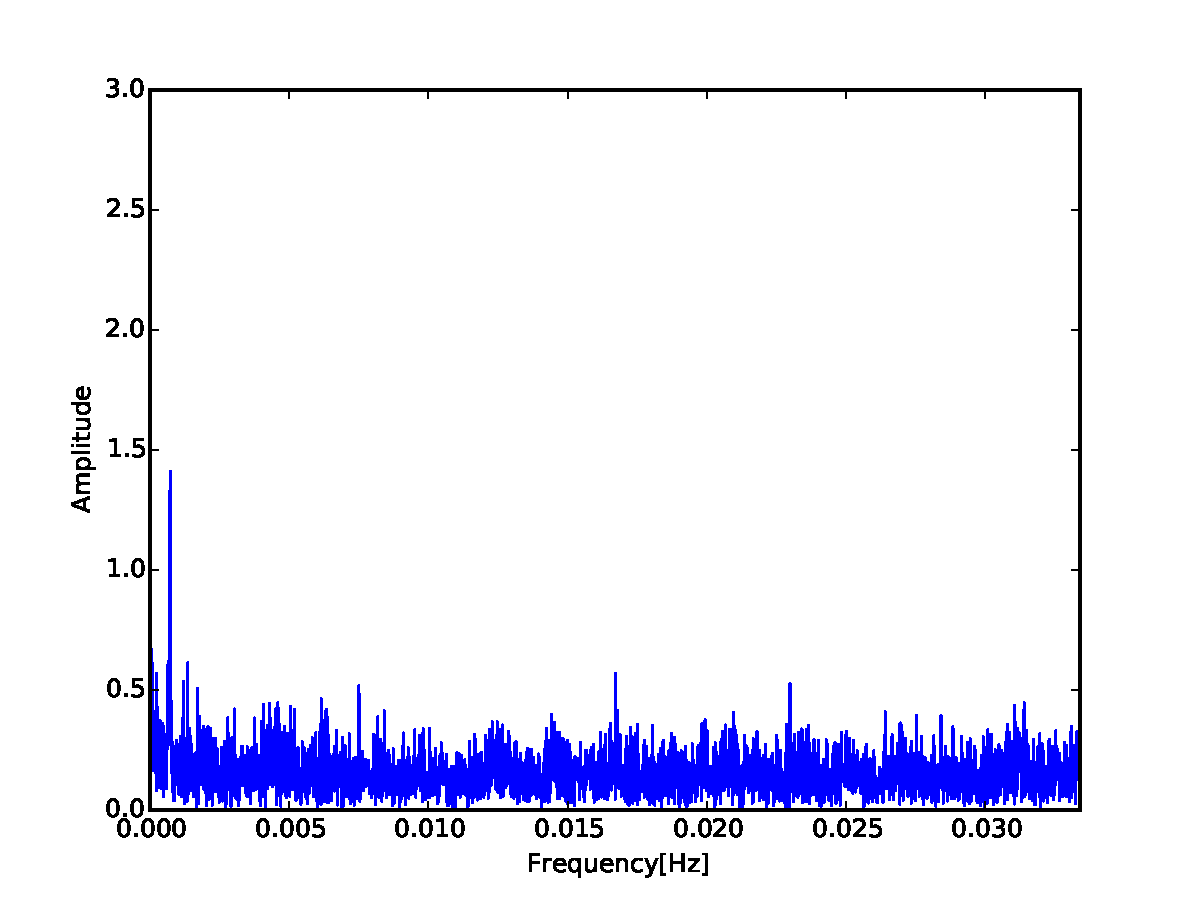
\includegraphics[width=0.33\hsize]{C:/master/mstudy/analysis/long/fft_6-23.pdf}
}~
\subfigure[6 月 24 日]{
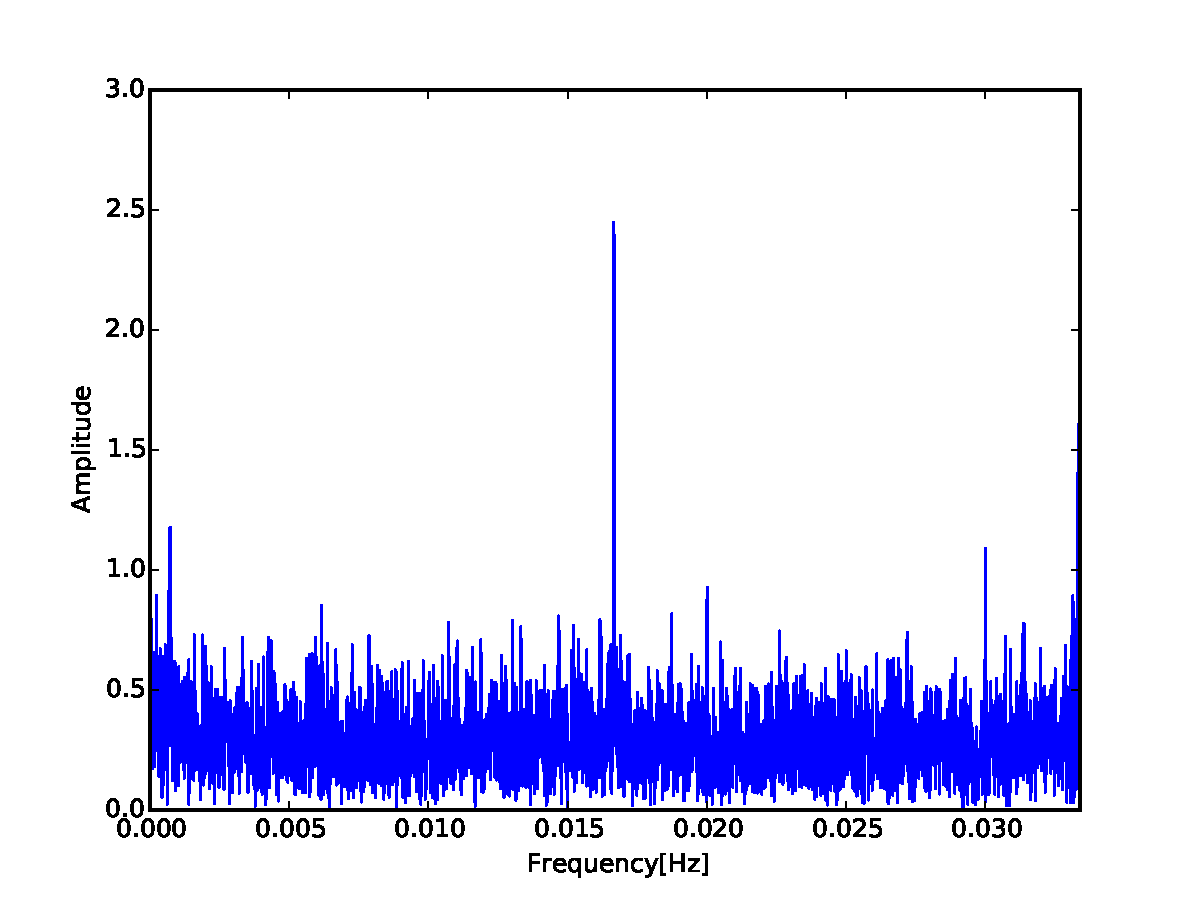
\includegraphics[width=0.33\hsize]{C:/master/mstudy/analysis/long/fft_6-24.pdf}
}~
\subfigure[6 月 25 日]{
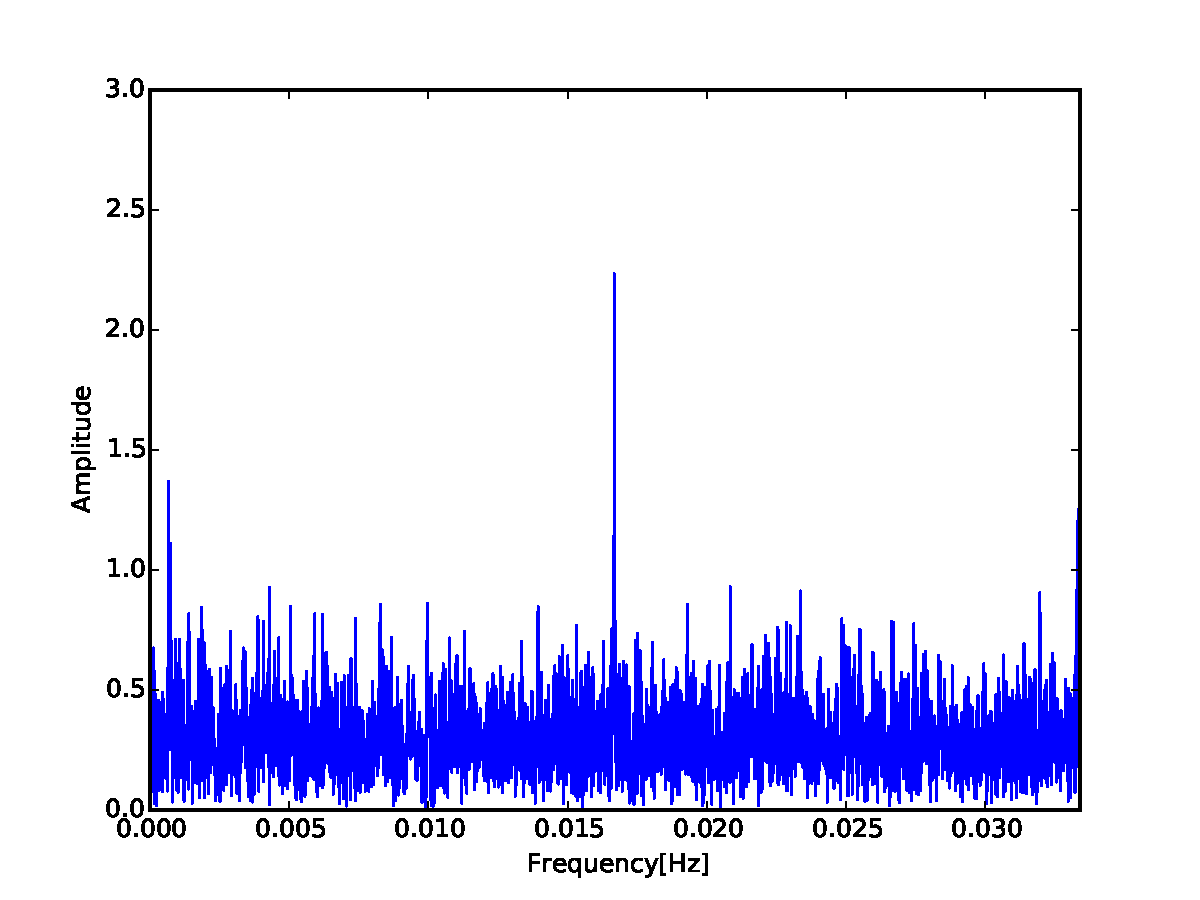
\includegraphics[width=0.33\hsize]{C:/master/mstudy/analysis/long/fft_6-25.pdf}
}
\caption{FFT}
\label{fft}
\end{center}
\end{figure}
図 \ref{fft} より,約 0.0007[Hz](約 24 分)の周波数成分が三つの区間データともに高いことがわかる.図 \ref{all1}(a),(b),(c) から小さな応答遅延の値が時間経過とともに増加する傾向を示す区間の時間的長さは約 30 分程度に見えるため,この周波数成分が知りたい区間の長さに対応すると考えられる.しかしながら一方で,6 月 24 日,6 月 25 日では約 0.017Hz(約 1 分)の周波数成分も大きく出ているため,元データから低遅延帯の波形のみを抽出したよりピンポイントな波形に対する FFT 分析が必要があると考えた.そこで次に,この三つの区間データそれぞれに対し,平均値以下の応答遅延を結んだ波形から移動平均(平滑化パラメータ 0.8)を取った図 \ref{low} の赤線で示す波形に FFT を適用した.その結果を図 \ref{lowfft} に示す.この図から図 \ref{fft} と同様の 0.0007[Hz](約 24 分)の周波数成分が高いことが読み取れる.したがって,低遅延帯が増加傾向を示す長さは 24 分程度であると思われる.
\begin{figure}[tb]
\begin{center}
\subfigure[6 月 23 日]{
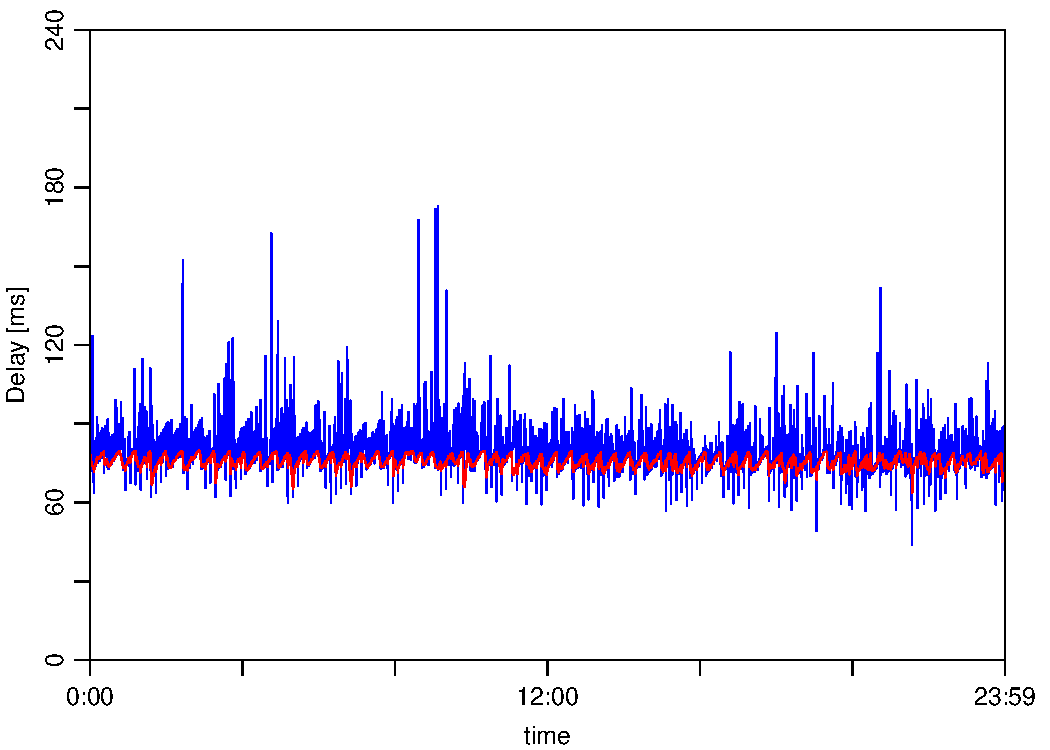
\includegraphics[width=0.5\hsize]{C:/master/mstudy/analysis/long/low_6-23.pdf}
}~
\subfigure[6 月 24 日]{
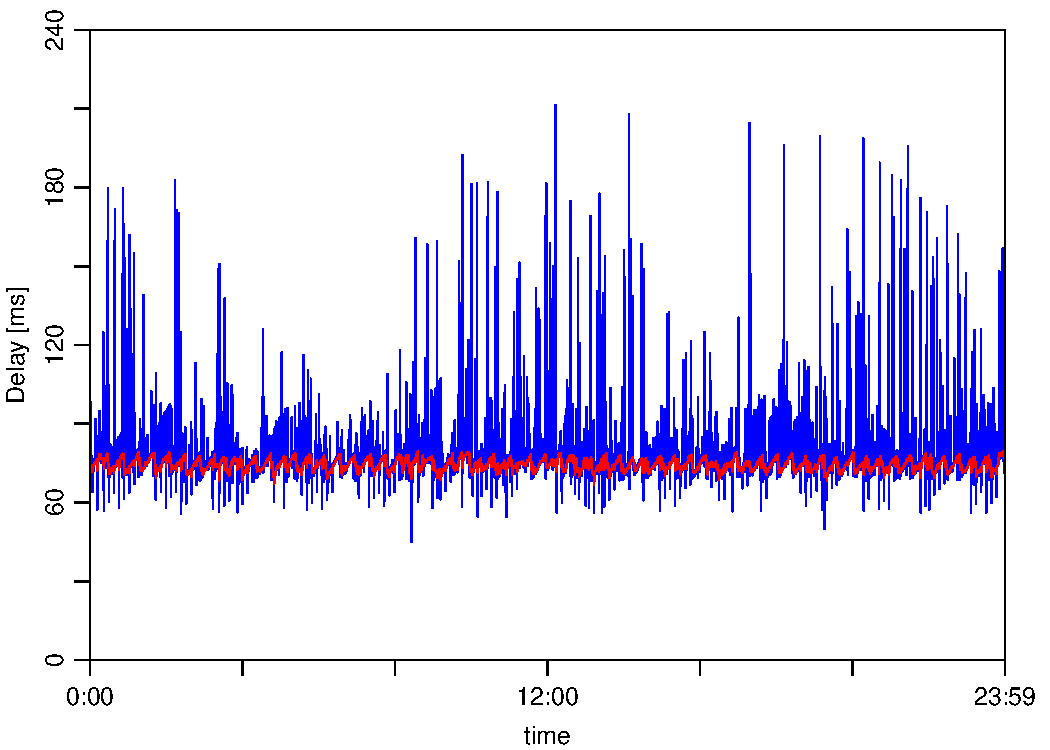
\includegraphics[width=0.5\hsize]{C:/master/mstudy/analysis/long/low_6-24.pdf}
}\\
\subfigure[6 月 25 日]{
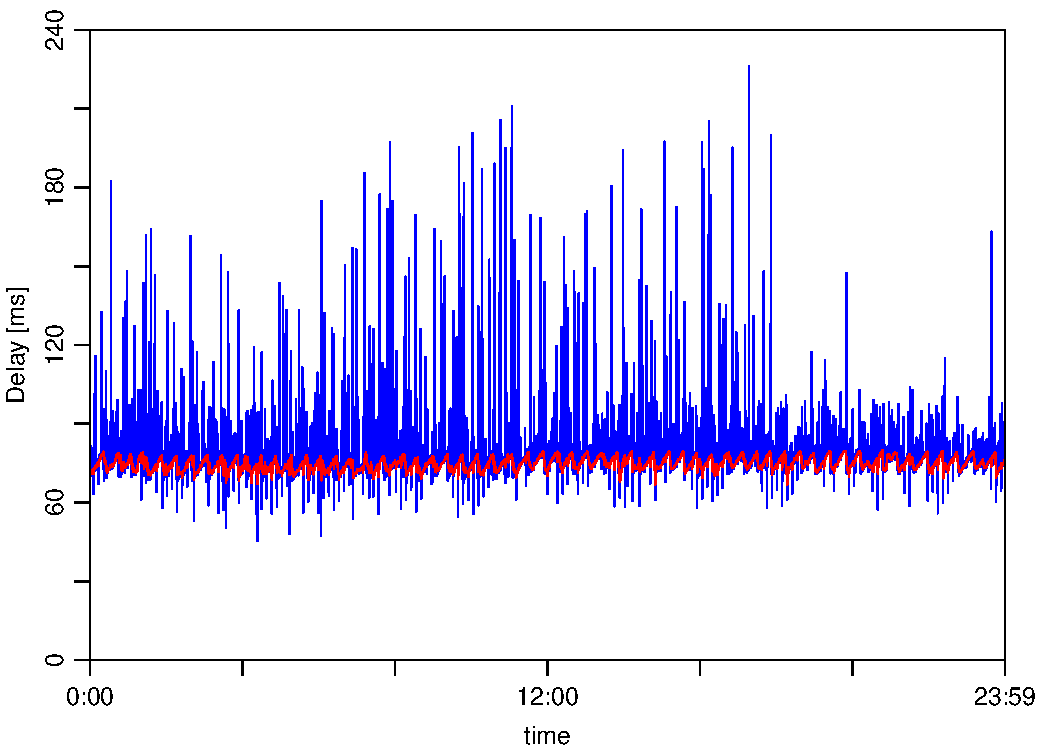
\includegraphics[width=0.5\hsize]{C:/master/mstudy/analysis/long/low_6-25.pdf}
}
\caption{低遅延帯の抽出}
\label{low}
\end{center}
\end{figure}
\begin{figure}[tb]
\begin{center}
\subfigure[6 月 23 日]{
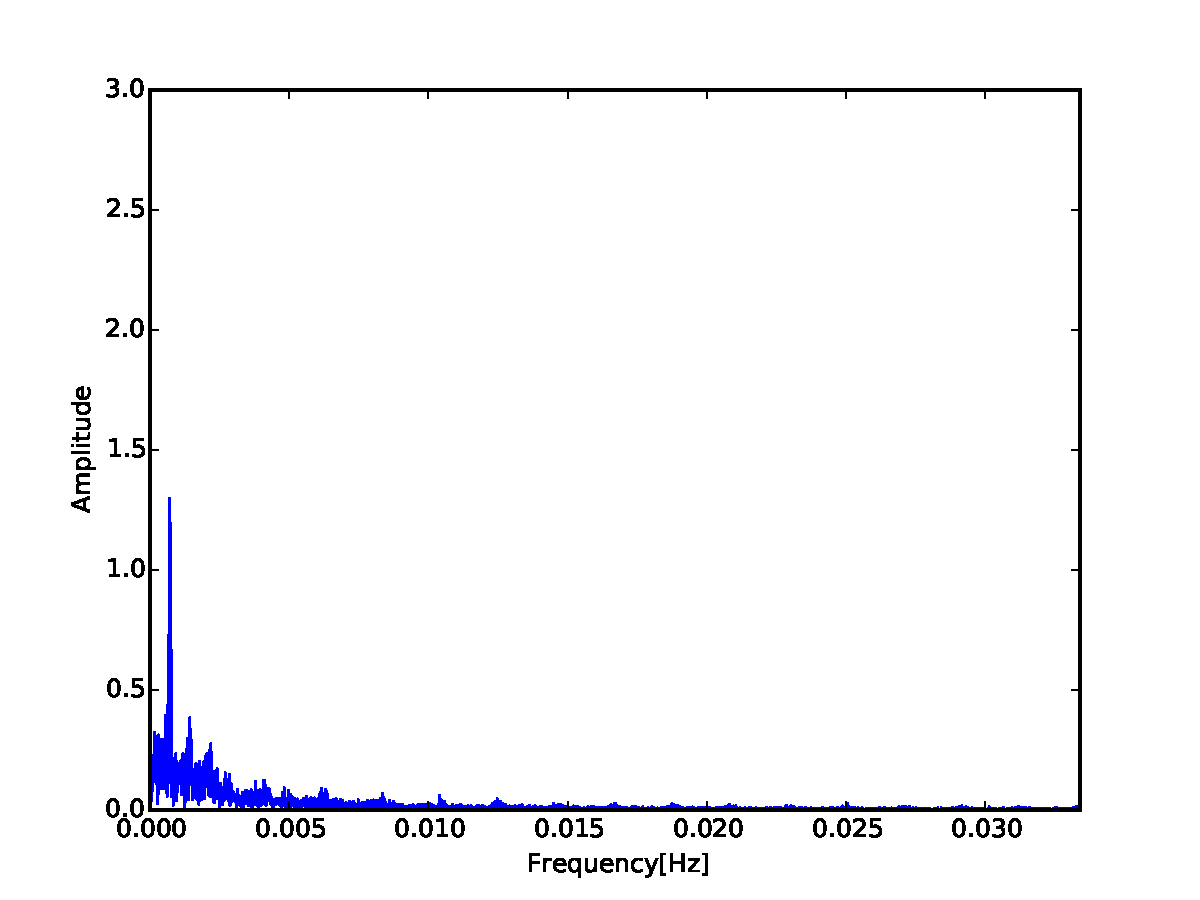
\includegraphics[width=0.33\hsize]{C:/master/mstudy/analysis/long/fft_low_6-23.pdf}
}~
\subfigure[6 月 24 日]{
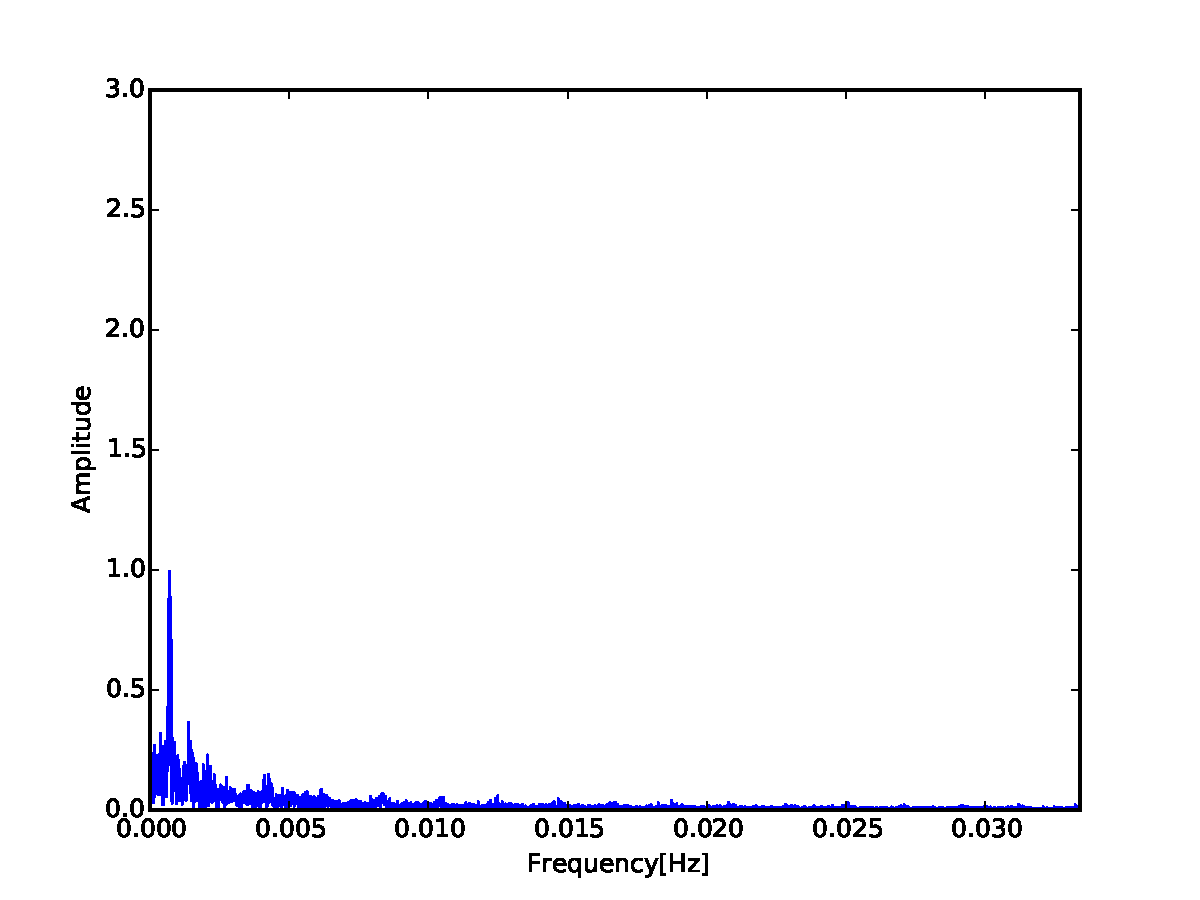
\includegraphics[width=0.33\hsize]{C:/master/mstudy/analysis/long/fft_low_6-24.pdf}
}~
\subfigure[6 月 25 日]{
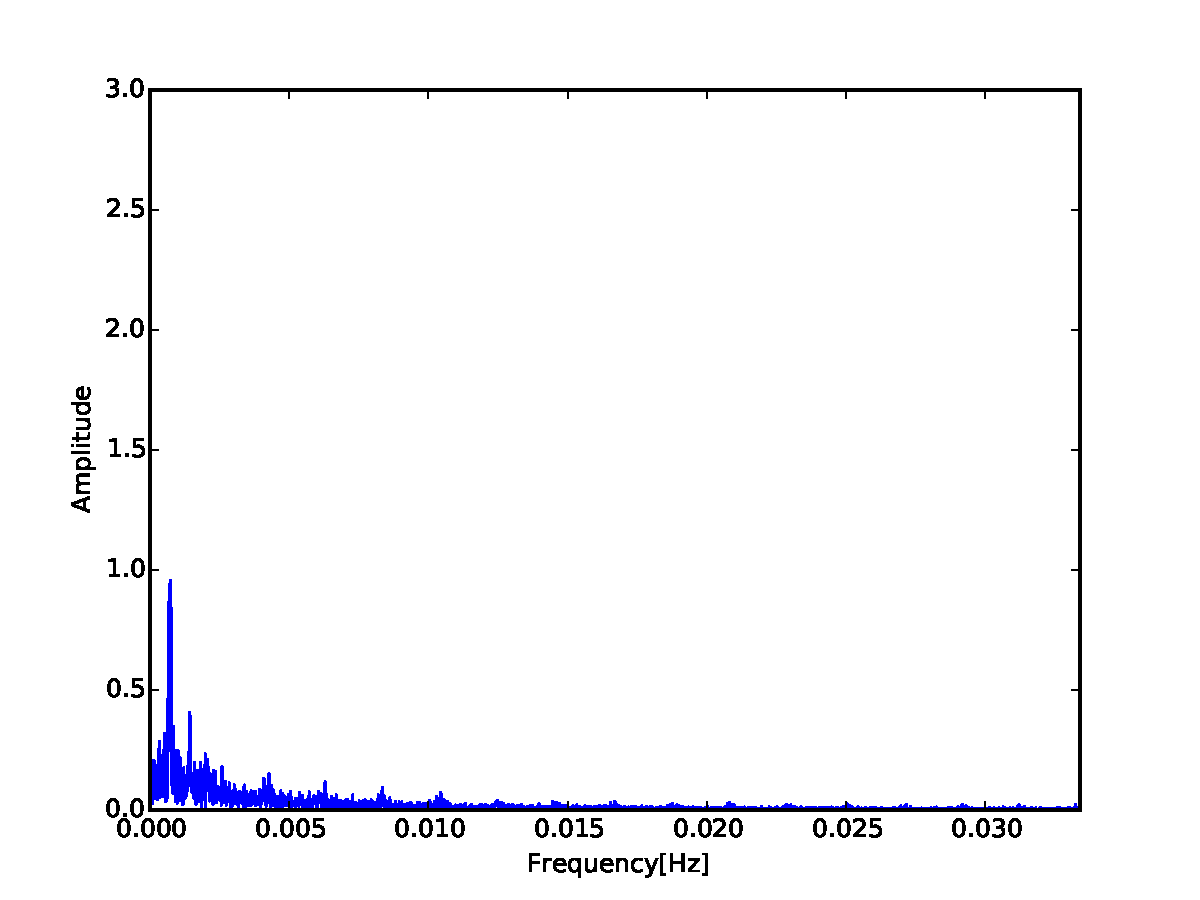
\includegraphics[width=0.33\hsize]{C:/master/mstudy/analysis/long/fft_low_6-25.pdf}
}
\caption{低遅延帯を抽出した波形に FFT を用いた結果}
\label{lowfft}
\end{center}
\end{figure}
\section{大きな応答遅延の発生要因箇所の切り分け}
10 ミリ秒間隔で 20 分間行った計測実験では,大きな応答遅延が発生する区間が確認されていた.
そこでここでは,その発生要因が Raspberry Pi と eNodeB との間にあるのか,eNodeB よりも向こう側にあるのかを切り分けるため,2 台の Raspberry Pi を近場に置き同 eNodeB に接続されていると考えられる環境下で,同時刻に 10 ミリ秒間隔での計測実験を行った.20 分間行った計測実験において,大きな応答遅延が発生している一部の区間を取り出した結果を図 \ref{comp} に示す.横軸の時刻幅を 1 秒とし,赤線と青線はそれぞれ異なる Rapsberry Pi で計測される ping 応答遅延である.
\begin{figure}[tb]
\begin{center}
\subfigure[]{
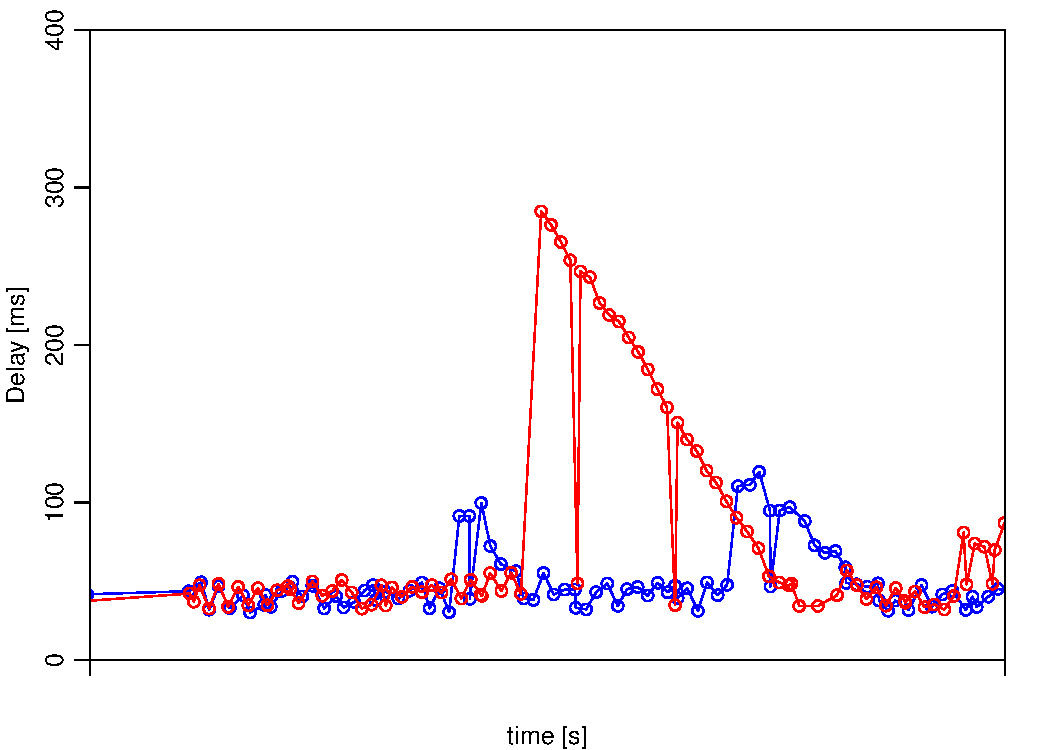
\includegraphics[width=0.33\hsize]{C:/master/mstudy/analysis/sequence/10ms/01_00.pdf}
}~
\subfigure[]{
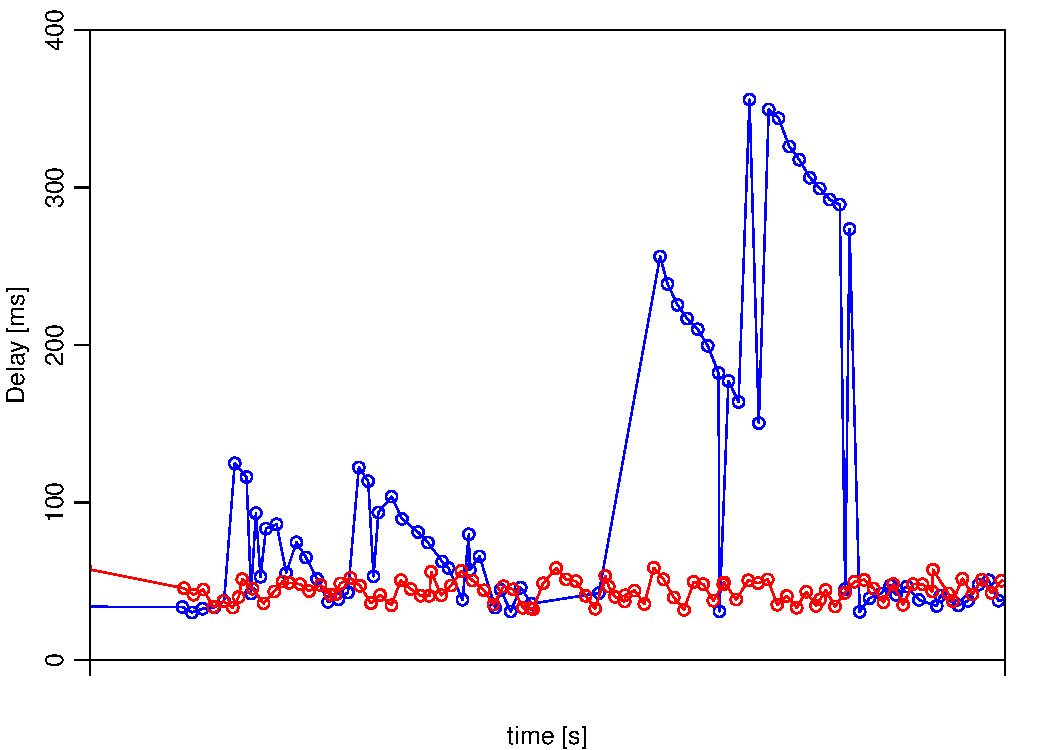
\includegraphics[width=0.33\hsize]{C:/master/mstudy/analysis/sequence/10ms/01_33.pdf}
}~
\subfigure[]{
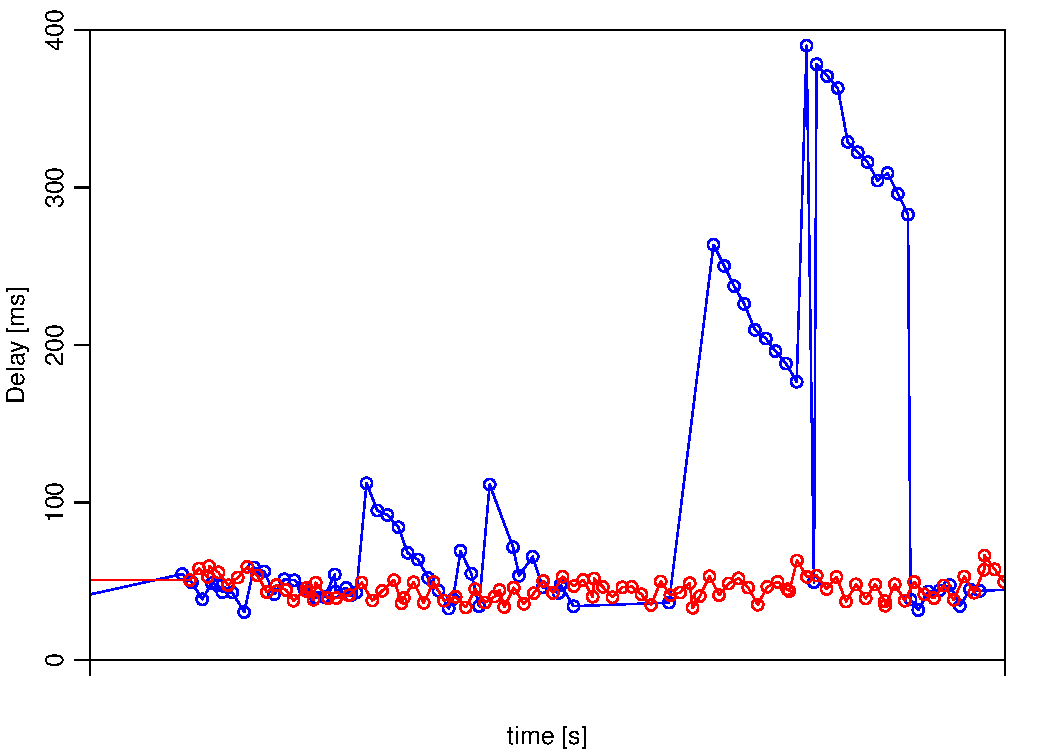
\includegraphics[width=0.33\hsize]{C:/master/mstudy/analysis/sequence/10ms/03_32.pdf}
}
\caption{端末間での応答遅延の比較}
\label{comp}
\end{center}
\end{figure}
図より,一方の端末で計測される応答遅延が大きくなる区間であっても,もう一方で大きな応答遅延が計測されるわけではないようだ.
つまり,この大きな応答遅延は各端末と eNodeB との間で発生するものと考えられる.
\end{document}